\section{Multivariate Analysis}%
\label{sec:multivariate_analysis}

The event selection described in~\Cref{sec:event_selection} serves as
a pre-selection to select events compatible with the expected final
state of the signal processes, and ensuring that basic requirements on
kinematic properties of final state objects are fulfilled. %
% , ensuring trigger efficiencies are in saturation,
The signal-to-background ratio at this level of selection, with
background being three orders of magnitude more abundant than the
expected non-resonant \HH signal in the \hadhad channel
(cf.~\Cref{tab:hadhad_presel_yields}), is not sufficient to provide
any signal sensitivity without further signal-background
discrimination.

The final state particles from non-resonant and resonant production of
Higgs boson pairs have distinct kinematic properties that can be used
to reject backgrounds in the signal region.
% An example, largely independent of the \HH production mode, is the
% reconstructed invariant mass of the $H \to \bbbar$ or
% $H \to \tautau$ candidate.
A number of reconstructed quantities can be defined that offer
discrimination power. These are exploited using multivariate methods
to classify events regarding their similarity to the signal process of
interest.
% Multivariate methods are then used to exploit these
% quantities and their correlations, classifying events regarding their
% similarity to the signal processes of interest.
Depending on the \HH production mode and analysis category, different
methods are used.

% Multivariate methods are used to exploit the discrimination power of
% multiple reconstructed quantities and their correlations, classifying
% events regarding their similarity to the signal and background
% processes. Depending on the \HH production mode and analysis category
% different methods are used.

The search for SM \HH production uses Boosted Decision Trees and
Neural Networks to distinguish signal from background events in the
\hadhad and \lephad channels, respectively. When searching for
resonant \HH production, multiple mass hypotheses for the scalar
resonance decaying into Higgs boson pairs are considered. The
kinematic properties of final state particles in signal events depend
on the mass of the resonance, \mX, and as a result the classification
task varies continuously with \mX. This contrasts the former case in
which the kinematic properties of signal events follow from a fixed
distribution predicted by the SM. Classification tasks that vary as a
function of a parameter, for example the mass of a resonance, can be
performed by \emph{Parameterised Neural Networks} (PNNs) which were first
introduced to HEP in Ref.~\cite{Baldi:2016fzo}. PNNs provide a single
classifier that is able to handle sets of classification tasks
described by one or more parameters. Therefore, they are used as
discriminants in the search for resonant \HH production in the \hadhad
and \lephad channels.
% while being able to smoothly interpolate to parameter values not
% seen during training of the network.

The scores provided by these multivariate classification methods,
hereafter called MVA scores, are later used as a discriminant in
maximum likelihood fits to extract the signal of interest and to set
upper limits on signal strengths and cross-sections. No further
selections are applied to events entering the signal extraction
procedure such that the pre-selection regions are also signal regions
of the respective channels. During the development of the analysis,
regions at high MVA scores were blinded to avoid selection biases.

In \Cref{sec:mva_discriminating variables} the choice of
discriminating variables used to classify signal and background events
is motivated. \Cref{sec:mva_crossvalidation} introduces a method used
to train, optimise, and evaluate classifiers that ensures that the
predicted MVA scores are unbiased and can be used in the statistical
interpretation of the search results. This method is employed in
\Cref{sec:mva_smbdt} and \Cref{sec:mva_pnn} to obtain BDT- and
PNN-based classifiers used to extract signal events in the \hadhad
channel.

% \Cref{sec:mva_crossvalidation} begins by describing the
% cross-validation method used to ensure that model selection and MVA
% predictions are unbiased. In~\Cref{sec:mva_discriminating variables}
% the choice of discriminating variables used to classify signal and
% background events will be motivated. Afterwards, the training and
% optimisation of the classifiers used to extract SM \HH signal is
% described in~\Cref{sec:mva_smbdt}. Finally, \Cref{sec:mva_pnn}
% describes the event classification using PNNs for the search for
% resonant production of \HH, including a brief discussion of their
% properties.


\subsection{Discriminating Variables}%
\label{sec:mva_discriminating variables}

The set of variables provided to the multivariate classification
methods is critical to their performance in distinguishing between
classes. The initial choice of variables considered in this search is
based on the previous publication by the ATLAS collaboration in the
same analysis channel~\cite{HIGG-2016-16-witherratum}. Only minor
changes to the input variable selection are performed for this search.

The distinct kinematic properties of Higgs boson pair production allow
to distinguish the signal processes from the main backgrounds in the
\bbtautau search channel. The four-momenta of
$\PHiggs \ra \Pbottom\APbottom$ and $\PHiggs \ra \tautau$ candidates
are reconstructed\footnote{The fraction of events with a
  misreconstructed $H \to \bbbar$ or $H \to \tautau$ candidate, i.e.\
  \btagged jets / \tauhadvis not being matched to Higgs boson decay
  products at generator-level, are about \SI{2}{\percent} and
  \SI{0.2}{\percent} in signal region of the \hadhad channel,
  respectively.}  and are used to define discriminating variables.
Among the most important variables are \PHiggs- and \HH-system
invariant masses:
\begin{description}

\item[\mBB] The invariant mass of the $H \to \bbbar$ candidate. It is
  reconstructed using the four-momenta of both \btagged jets in the
  signal regions after $b$-jet momentum corrections. The Higgs boson
  mass is reconstructed with a resolution of \SIrange{13}{18}{\GeV}
  for the signal processes considered in this search.

\item[\mMMC] The invariant mass of the $H \to \tautau$ candidate
  reconstructed by the MMC. In the \hadhad channel, the mass
  resolution of the MMC ranges from \SIrange{15}{18}{\GeV} depending
  on the signal process.

\item[\mHH] The invariant mass of the pair of Higgs bosons in signal
  events. It is determined from the sum of four-momenta of the $b$-jet
  candidates after momentum corrections and the $\tautau$-system
  four-momentum reconstructed using the MMC. For signal events in the
  \hadhad channel the relative mass resolution is
  \SIrange{8}{10}{\percent}.

\end{description}
The bias and resolution of the \PHiggs and \HH mass reconstruction is
summarised in~\Cref{fig:mass_reconstruction} for resonant \HH
production as a function of the resonance mass. The three invariant
masses are used as inputs to the MVAs in the \hadhad and \lephad
channels.

% The performance of the \PHiggs candidate mass reconstruction is
% summarised in~\Cref{fig:mass_reconstruction_H} for the resonant
% production of \HH as a function of the resonance mass. The Higgs boson
% mass peaks in the \mMMC and \mBB spectra allow to select signals with
% high efficiency while providing large rejection power against most SM
% backgrounds. Both \PHiggs-system masses are used as inputs to the MVAs
% in all analysis channels.

% mHH:
% It provides an important discriminant in the search for resonant \HH
% production at high \mX.

% In the signal region of the \hadhad channel, the $H \to \tautau$
% candidate is reconstructed correctly for most signal events. The
% fraction of events where the candidate is misreconstructed is about
% \SIrange{0.1}{0.2}{\percent}. The fraction of signal events with a
% misreconstructed $H \to \bbbar$ candidate is about \SI{2}{\percent}
% and increases to a maximum of \SI{5}{\percent} for events from scalar
% resonances with $\mX = \SI{1600}{\GeV}$.\todo{Move to somewhere else?}


\begin{figure}[htbp]
  \centering

  \begin{subfigure}[t]{.5\textwidth}
    \centering
    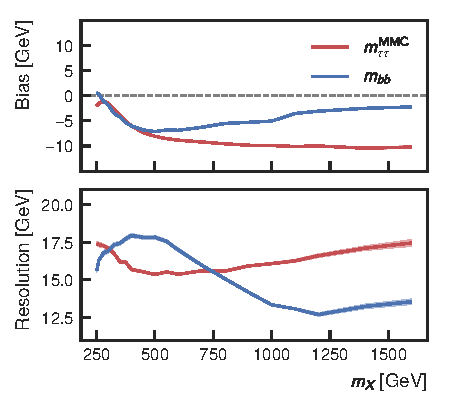
\includegraphics{mva/mass_resolution}
    \subcaption{\PHiggs-system mass reconstruction}
    \label{fig:mass_reconstruction_H}
  \end{subfigure}\hfill%
  \begin{subfigure}[t]{.5\textwidth}
    \centering
    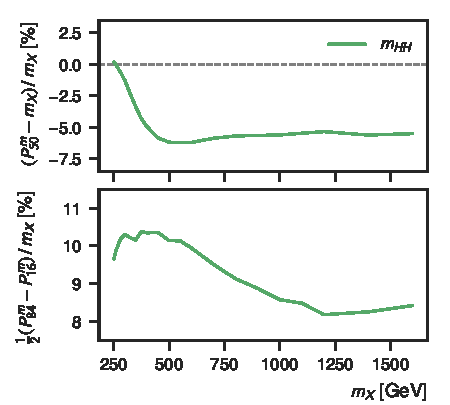
\includegraphics{mva/mhh_resolution}
    \subcaption{\HH-system mass reconstruction}
    \label{fig:mass_reconstruction_HH}
  \end{subfigure}

  \caption{Performance of methods used to reconstruct the
    \PHiggs-system mass (a) and the \HH-system mass (b) in the \hadhad
    signal region estimated using simulation of
    $\PX \ra \HH \ra \bbtautau$ processes. The top panels show the
    bias of the mass prediction given in terms of deviation of the
    median mass prediction from the true mass value. The bottom panels
    show the mass resolution estimate as half of the length of the
    central interval containing \SI{68}{\percent} of all mass
    predictions. For the \HH-system mass reconstruction shown in (b),
    the bias and resolution is given relative to the mass of the
    resonance.}%
  \label{fig:mass_reconstruction}
\end{figure}

Higgs bosons originating from signal processes are typically produced
with large momenta in the \HH rest frame, the exception being resonant
\HH production \mX close to the \HH production threshold, thus leading
to a small separation of the (visible) \PHiggs decay products. The
distances \dRtautau and \dRbb between the visible decay products of
the \tauleptons and $b$-jet candidates, respectively, provide
discrimination power against multi-jet and top quark pair production
where \tauleptons and $b$-jet candidates are less collimated. Both
variables are used as inputs to the MVAs in the \hadhad and \lephad
SLT channel.

In a given analysis channel, the same set of input variables is used
for the search for non-resonant and resonant \HH production. The
choice of variables between channels differs and is summarised
in~\Cref{tab:mva_inputvar}. The five discriminating variables used in
the \hadhad channel are shown in~\Cref{fig:mva_inputs}.
% A selection of variables used in the \lephad SLT and LTT channels
% are documented in Ref.~\cite{ATLAS-CONF-2021-030}.

\begin{table}[htbp]
  \centering

  \caption{Input variables of the multivariate classifiers used in the
    \hadhad and \lephad channels. The same variables are used for the
    search for SM \HH and resonant \HH production. Definitions of the
    input variables used in the \lephad channels are given in
    \Cref{app:lephad_mva_variables}. The table is adapted from
    Ref.~\cite{ATLAS-CONF-2021-030}.}%
  \label{tab:mva_inputvar}

  \renewcommand{\arraystretch}{1.1}%
  \begin{tabular}{
  l
  >{\centering\arraybackslash}p{2cm}
  >{\centering\arraybackslash}p{2cm}
  >{\centering\arraybackslash}p{2cm}
  }
  \toprule
  & \multicolumn{3}{c}{Analysis Channel} \\ \cmidrule{2-4}
  Variable                              & \hadhad    & \lephad SLT & \lephad LTT \\
  \midrule
  \mMMC                                 & \checkmark & \checkmark & \checkmark \\[0.1em]
  \mBB                                  & \checkmark & \checkmark & \checkmark \\[0.1em]
  \mHH                                  & \checkmark & \checkmark & \checkmark \\[0.1em]
  \dRtautau                             & \checkmark & \checkmark & \checkmark \\[0.1em]
  \dRbb                                 & \checkmark & \checkmark &            \\[0.1em]
  $\Delta \pT(\ell, \tauhadvis)$        &            & \checkmark & \checkmark \\[0.1em]
  Sub-leading $b$-jet \pT               &            & \checkmark &            \\[0.1em]
  \mTW                                  &            & \checkmark &            \\[0.1em]
  \pTmissAbs                            &            & \checkmark &            \\[0.1em]
  \pTmiss $\phi$ centrality             &            & \checkmark &            \\[0.1em]
  $\Delta\phi(\ell\tauhadvis, bb)$      &            & \checkmark &            \\[0.1em]
  $\Delta\phi(\ell, \pTmiss)$           &            &            & \checkmark \\[0.1em]
  $\Delta\phi(\pTauTau, \pTmiss)$       &            &            & \checkmark \\[0.1em]
  $s_{\text{T}}$                         &            &            & \checkmark \\
  \bottomrule
 \end{tabular}


%%% Local Variables:
%%% mode: latex
%%% TeX-master: "../phd_thesis.tex"
%%% End:

\end{table}

% The \pTmiss $\phi$ centrality, previously used in the \hadhad
% channel~\cite{HIGG-2016-16-witherratum}, was not found to contribute
% to the classification performance when comparing models with cross
% validation in the \hadhad channel. It is therefore removed as an
% input to the multivariate discriminants of the \hadhad channel.

\begin{figure}[htbp]
  \centering

  \begin{subfigure}[t]{.46\textwidth}
    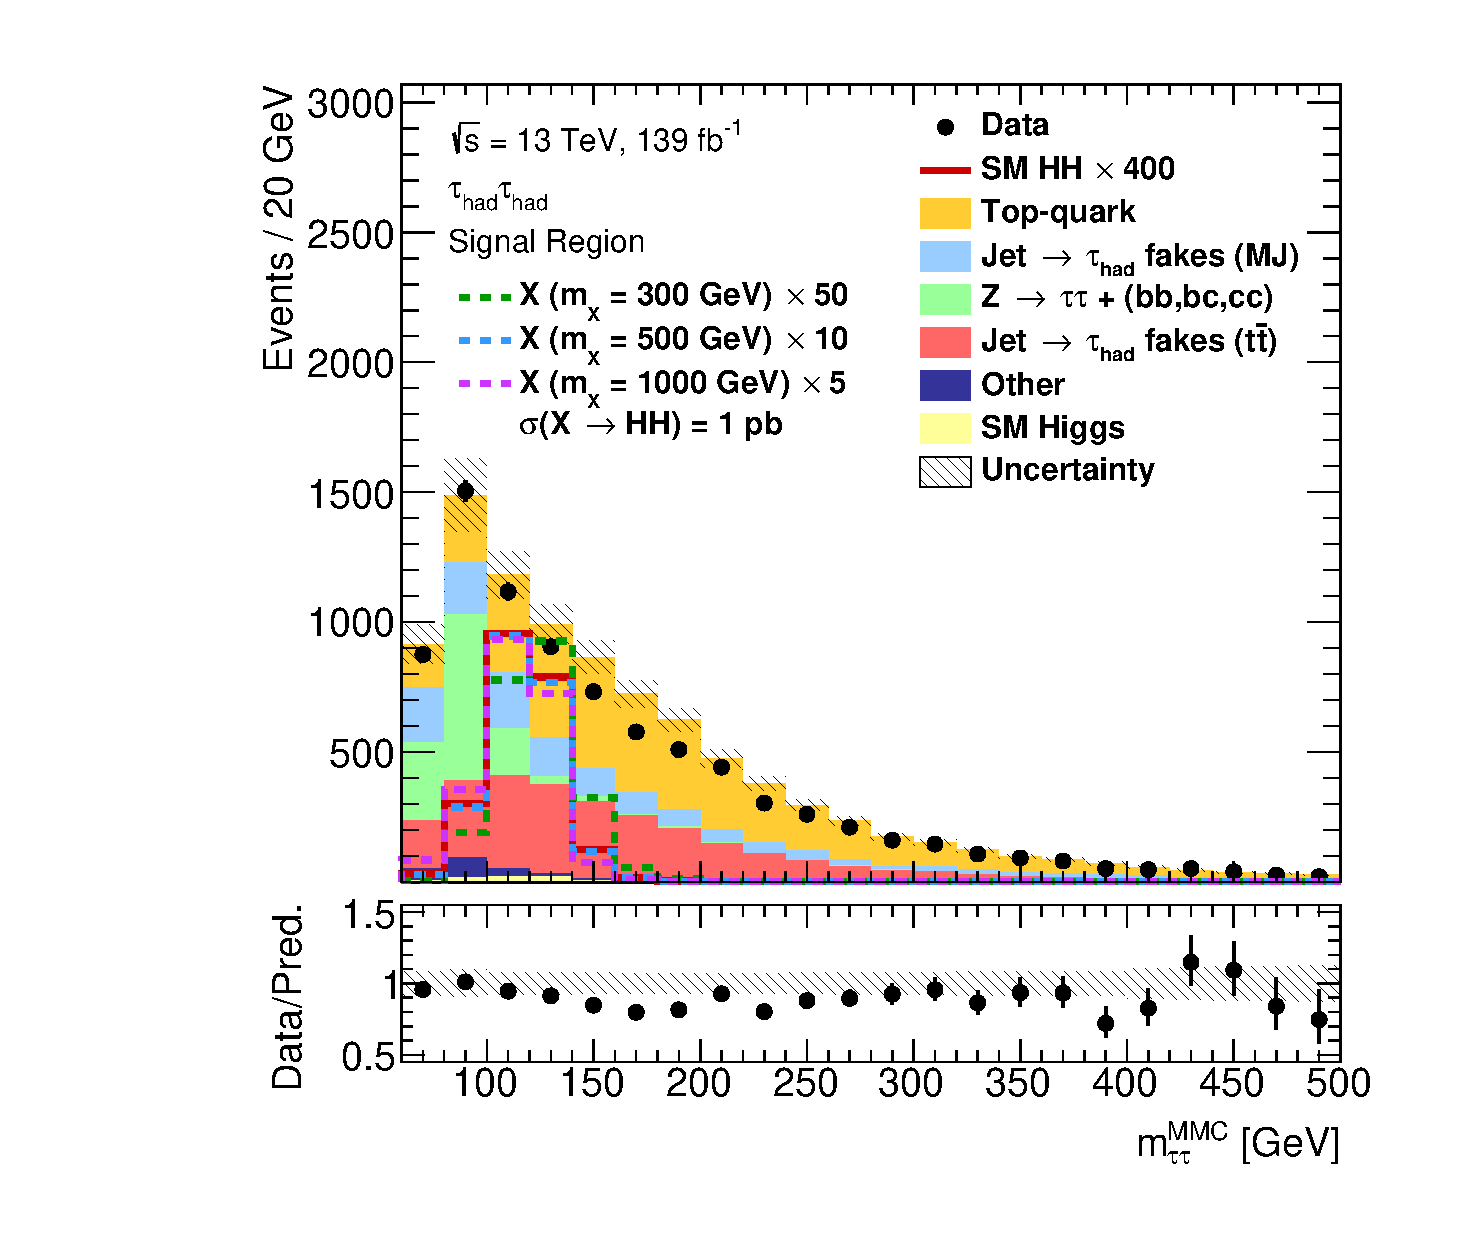
\includegraphics[width=\textwidth]{mva/prefit/Region_BMin0_incJet1_distmMMC_J2_Y2015_DLLOS_T2_SpcTauHH_L0_Prefit}
  \end{subfigure}\hfill %
  \begin{subfigure}[t]{.46\textwidth}
    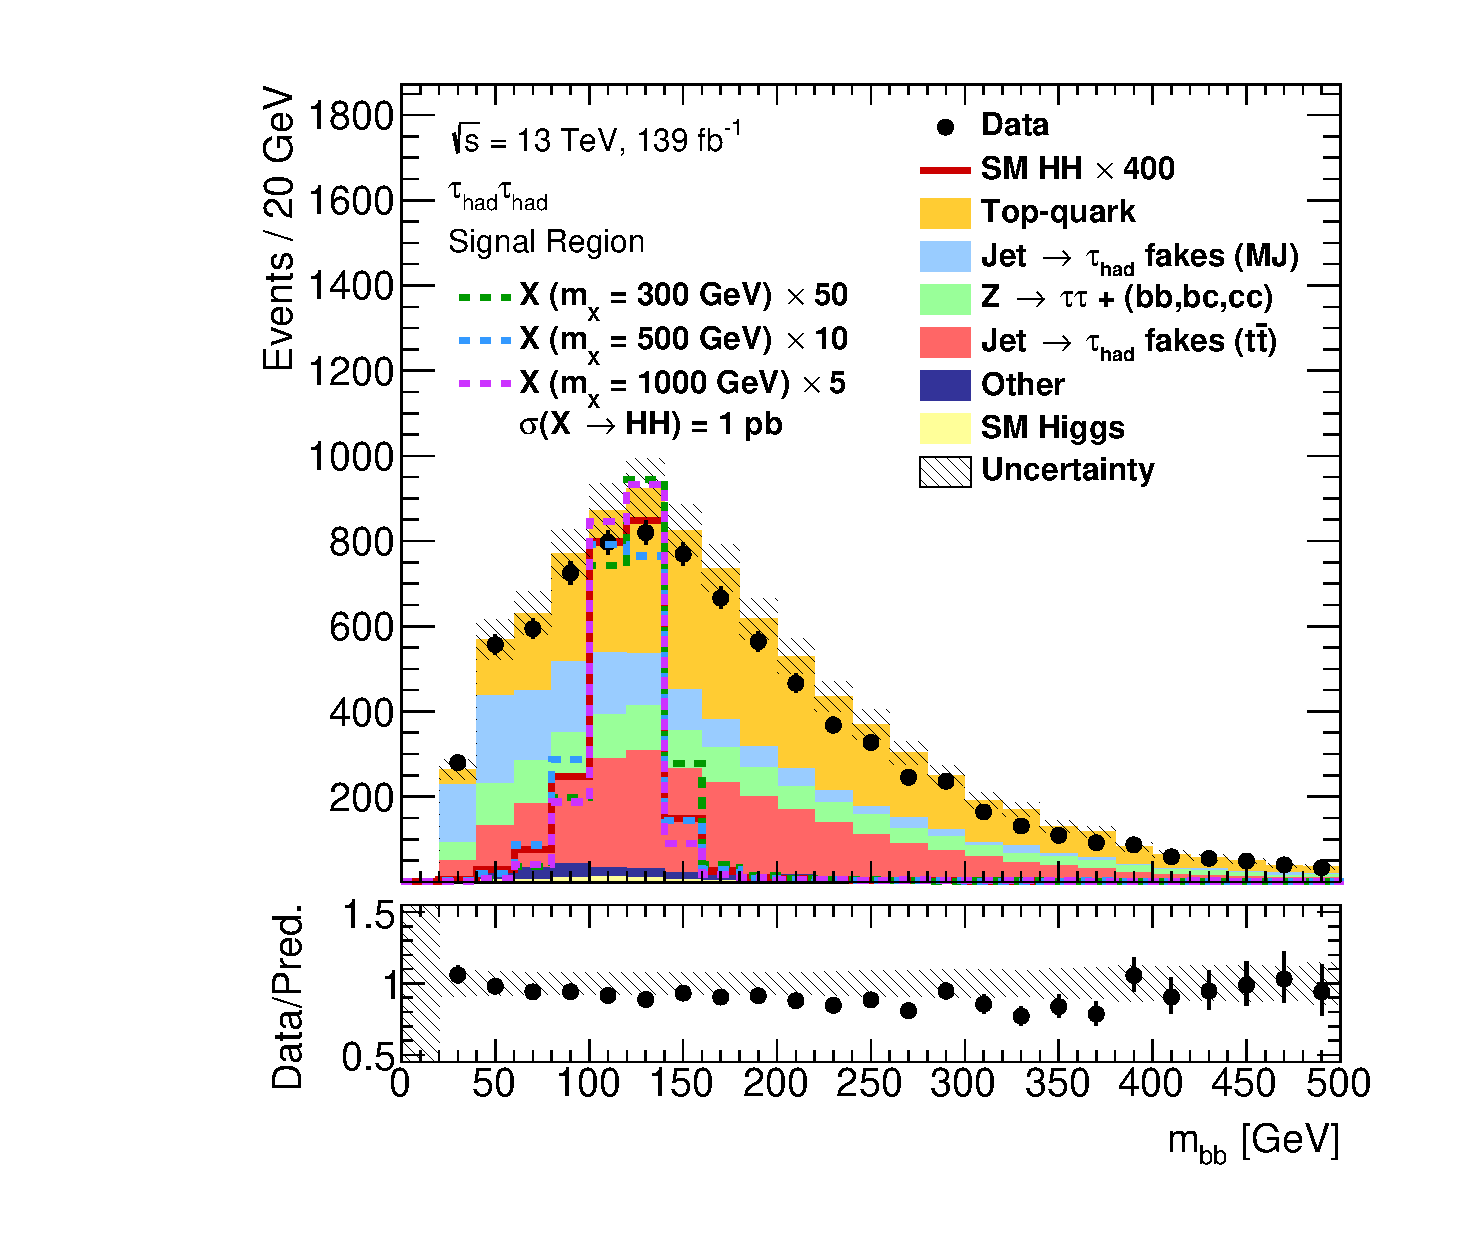
\includegraphics[width=\textwidth]{mva/prefit/Region_BMin0_incJet1_distmBB_J2_Y2015_DLLOS_T2_SpcTauHH_L0_Prefit}
  \end{subfigure}

  \begin{subfigure}[t]{.46\textwidth}
    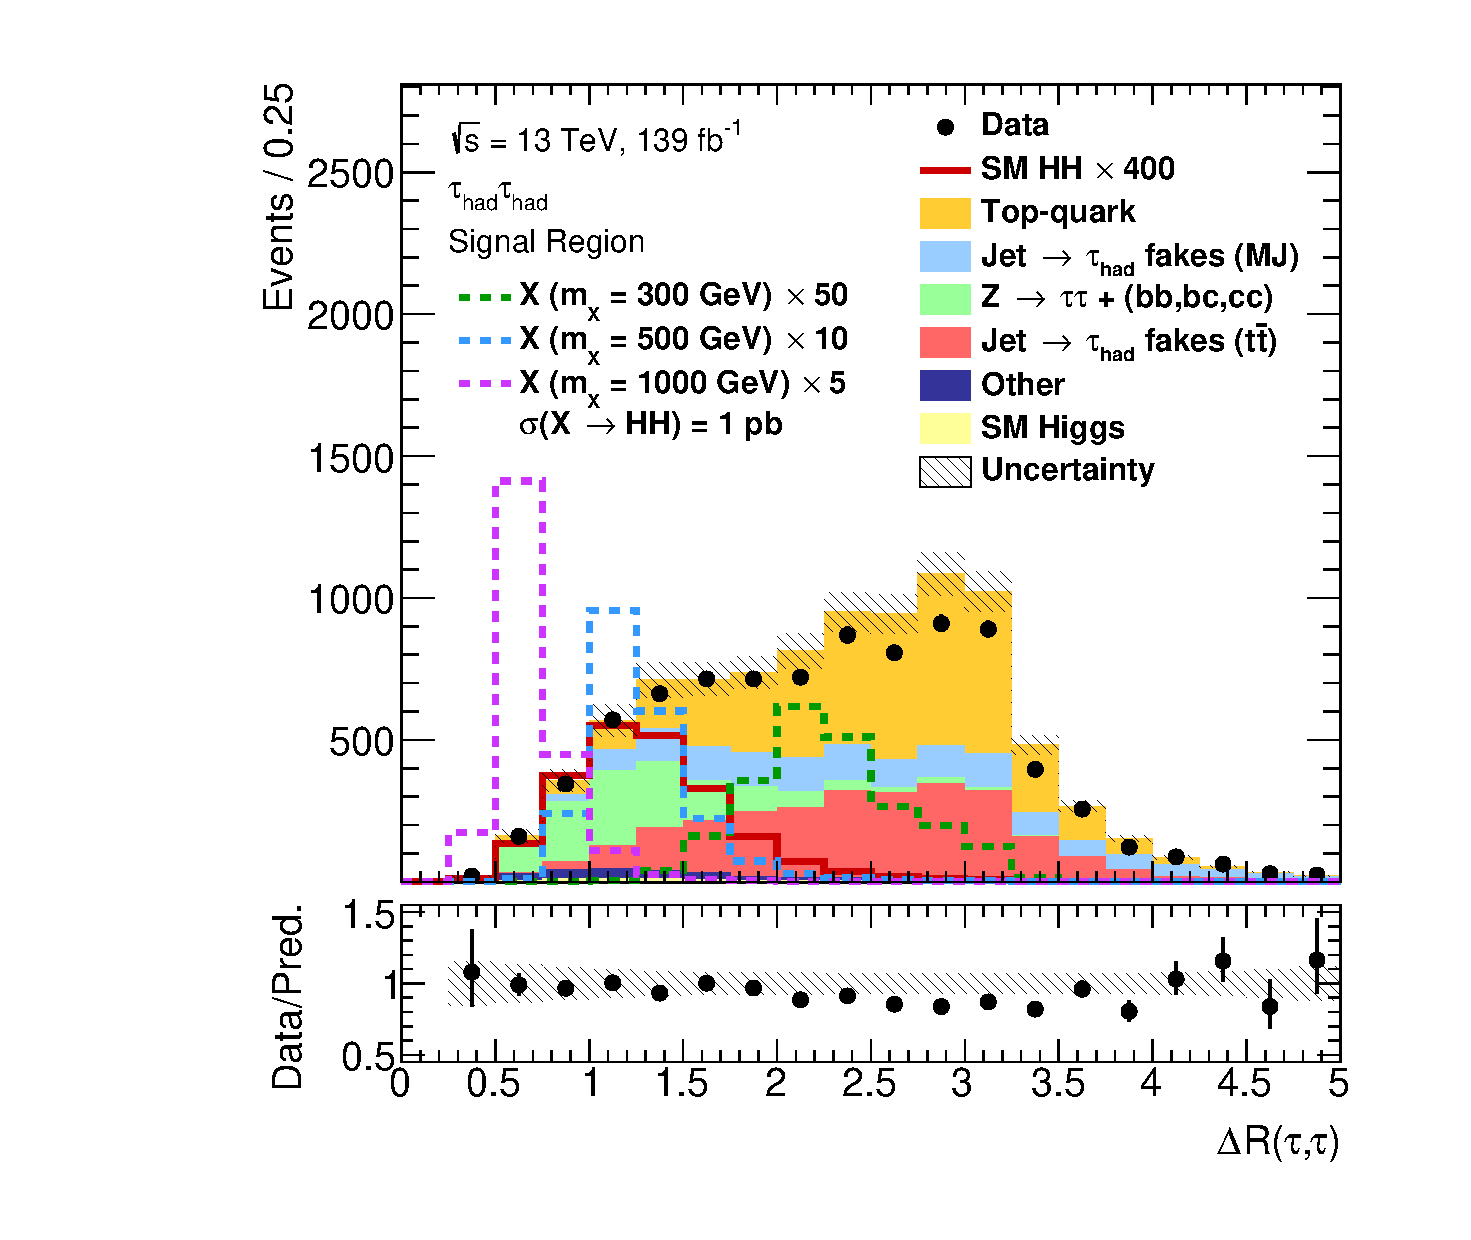
\includegraphics[width=\textwidth]{mva/prefit/Region_BMin0_incJet1_distdRTauTau_J2_Y2015_DLLOS_T2_SpcTauHH_L0_Prefit}
  \end{subfigure}\hfill %
  \begin{subfigure}[t]{.46\textwidth}
    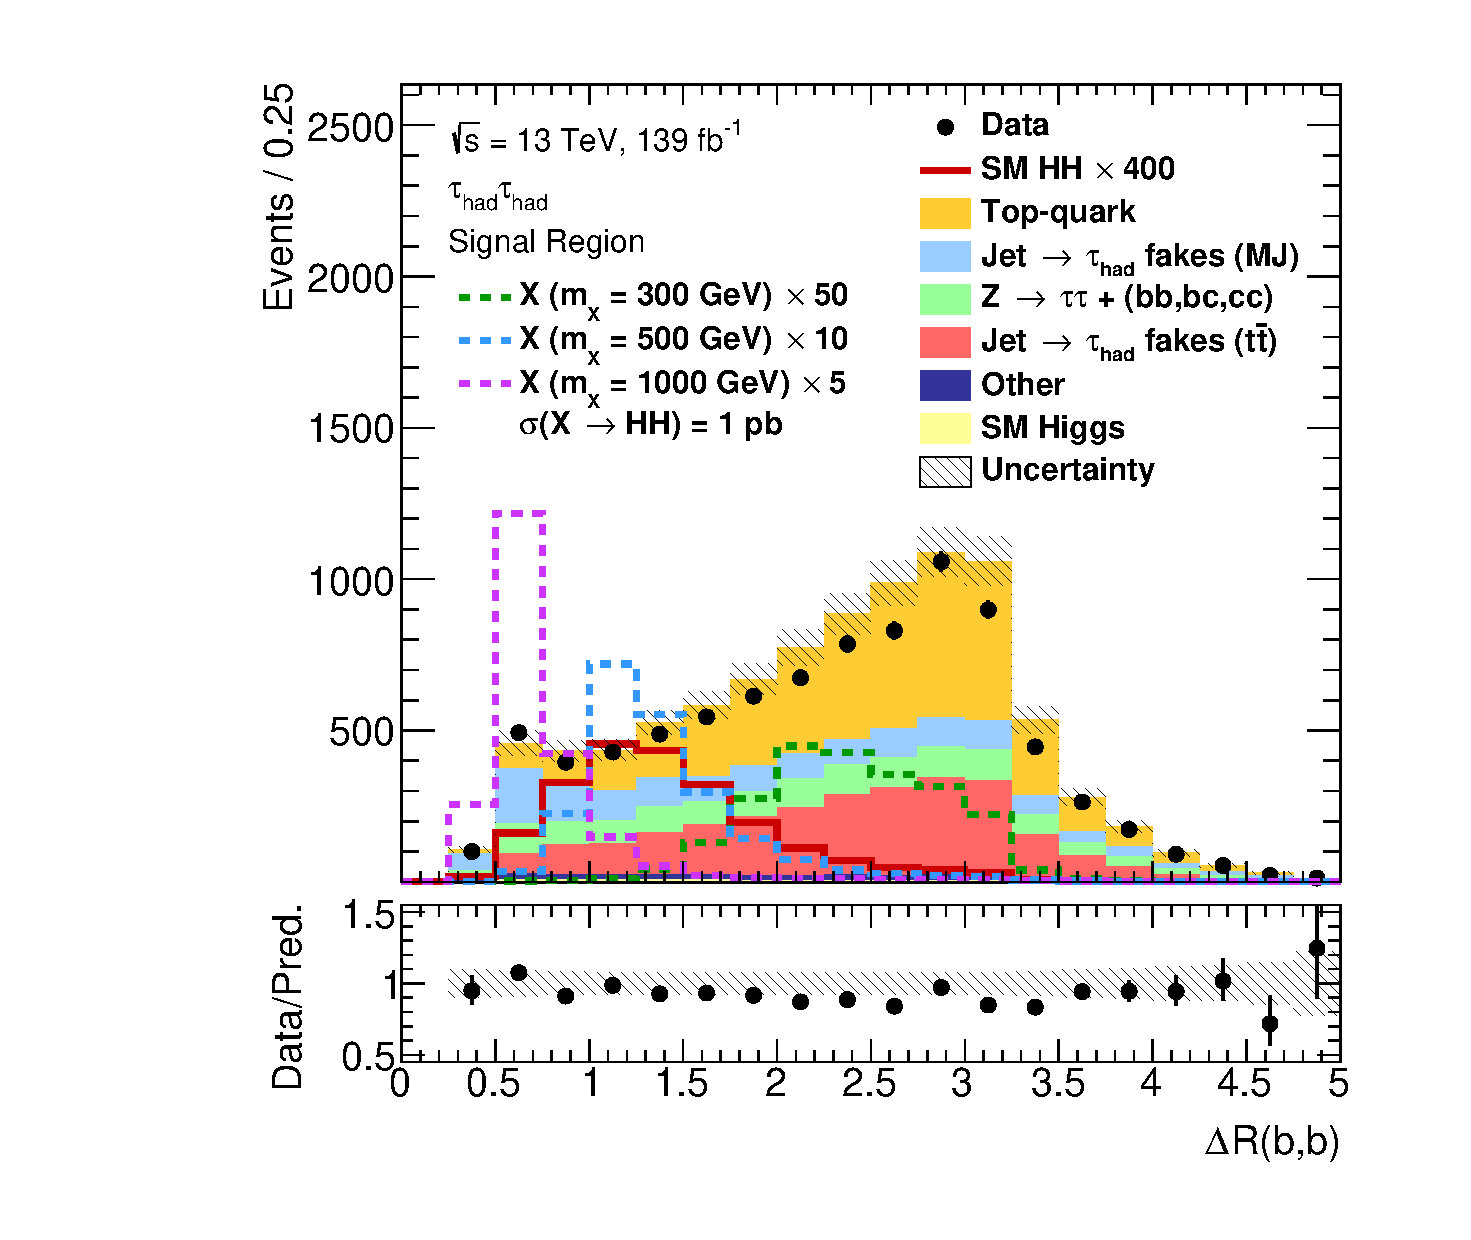
\includegraphics[width=\textwidth]{mva/prefit/Region_BMin0_incJet1_distdRBB_J2_Y2015_DLLOS_T2_SpcTauHH_L0_Prefit}
  \end{subfigure}

  \begin{subfigure}[t]{.46\textwidth}
    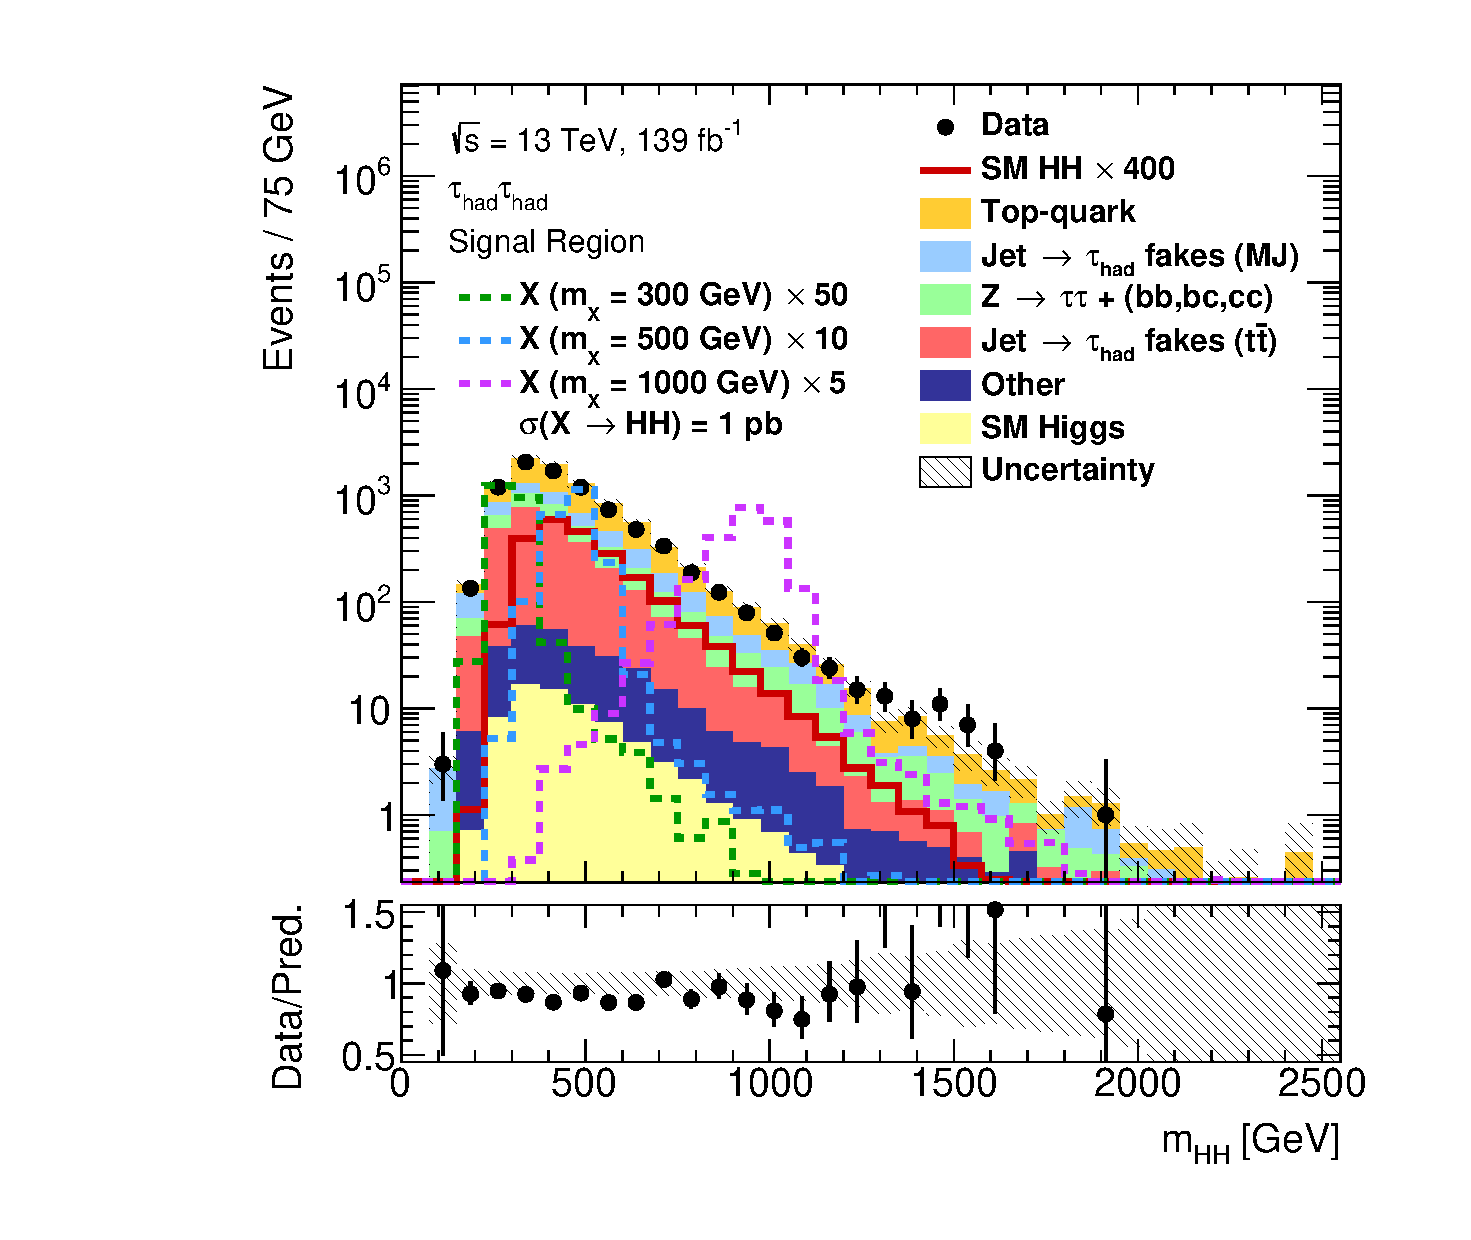
\includegraphics[width=\textwidth]{mva/prefit/Region_BMin0_incJet1_distmHH_J2_Y2015_DLLOS_T2_SpcTauHH_L0_Prefit_logy}
  \end{subfigure}

  \caption{Distributions of the MVA input variables in the signal
    region of the \hadhad channel prior to the maximum likelihood
    fit. The uncertainty bands include all statistical and systematic
    uncertainties of the background model. The normalisation of the
    resonant and non-resonant \HH signals are scaled for visibility.}%
  \label{fig:mva_inputs}
\end{figure}


\subsection{Cross-Validation Method}
\label{sec:mva_crossvalidation}

Many machine learning algorithms
% , due to their ability to approximate large classes of functions,
are susceptible to fitting statistical fluctuations in the data that
are used to train a model. As a result, predictions of performance
characteristics of the model based on the training data might not
generalise to previously unseen data. In extreme cases, frequently
called overfitting, the performance of the model evaluated on an
independent dataset starts to degrade when further increasing the
capacity of the model~\cite{hastie09}.

When using machine learning methods in searches for new physics, it
has to be ensured that the methods are evaluated on datasets that were
not used for training or model selection,\footnote{Model selection
  refers to the process of choosing a model from a set of models based
  on an evaluation metric.} thus providing an estimate of the
generalised performance. In this analysis, events are categorised
according to their event number into even- and odd-numbered
events. This two-fold split of events yields an even- and odd-fold,
respectively. The training and model selection can proceed by using
one of the two folds withholding the remaining fold for later
evaluation. This procedure is applied twice by using each fold for
training and model selection once.

Predictions of the MVA scores are obtained by evaluating the model
trained on the even- on odd-numbered events and the model trained on
the odd- on even-numbered events. This approach, which is called
2-fold \emph{cross-validation}~\cite{hastie09,bishop06}, provides
unbiased predictions of the MVA scores for the entirety of the
available dataset. The same evaluation method is applied to signal
region data recorded by the ATLAS detector. After assigning MVA scores
to all events, no distinction is made between even- and odd-numbered
events for the remainder of the analysis.

% The models are evaluated by applying the model trained on the
% even-fold on odd-numbered events and the model trained on the odd-fold
% on even-numbered events. This approach, which is called 2-fold
% \emph{cross-validation}~\cite{hastie09,bishop06}, provides an unbiased
% evaluation of the MVA scores using the entirety of the available
% dataset. The same evaluation method, including the separate treatment
% of even- and odd-numbered events, is applied to signal region data
% recorded by the ATLAS detector.

Similar to the biased predictions obtained when evaluating machine
learning methods on datasets used for training, the process of model
selection needs to be performed on a dataset that is independent of
the one used for final evaluation~\cite{cawley10}. In the case of this
analysis, model selection primarily applies to the determination of
the hyperparameters of the classification algorithms based on a
performance metric. Making this choice dependent on the performance on
the withheld dataset can introduce a selection bias when using the
same dataset for the statistical interpretation.

In this search, model selection is performed using 5-fold
cross-validation (CV), a generalisation of the 2-fold approach to a
larger number of subdivisions, separately on even- and odd-numbered
events. This approach effectively nests 5-fold CV inside 2-fold CV and
is therefore called \emph{nested cross
  validation}~\cite{cawley10,stone74}.

\Cref{fig:cross_validation} shows a schematic description of one
iteration of the nested cross-validation approach. The inner, 5-fold
CV randomly partitions events into five folds. For every choice of
evaluation-fold, the model is trained on the remaining four folds and
subsequently evaluated on the evaluation-fold. A decision between two
competing models can be made by comparing the average and standard
deviation of an evaluation metric over the five iterations of the inner
CV. Only after the best-performing model is selected, usually after
re-fitting the model on the combination of all five folds, it is
evaluated on the hold-out dataset.

\begin{figure}[htbp]
  \centering

  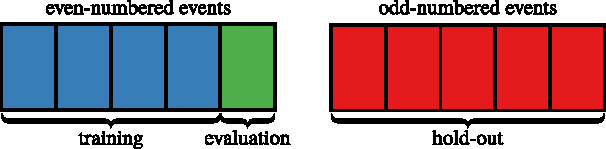
\includegraphics[scale=1]{mva/kfold}

  \caption{5-fold cross-validation approach for model selection on
    even-numbered events. The separation of events into disjoint
    subsets (folds) is indicated by rectangles. The purpose of the
    subset is denoted below. A single step out of a total of five, the
    number of possible assignments of the evaluation-fold, is
    shown. The hold-out dataset consisting of odd-numbered events is
    not used when performing model selection on even-numbered
    events.}%
  \label{fig:cross_validation}
\end{figure}



\subsection{Extraction of Signals from SM \HH Production with BDTs in
  the \hadhad Channel}%
\label{sec:mva_smbdt}

The search for SM \HH production in the \hadhad channel uses BDTs to
separate signal from background events. Events passing the signal
region selection (2~$b$-tag region) of the \hadhad channel are used to
train BDT. The training considers the non-resonant \HH production via
\ggF as the \emph{signal class}; the combination of all backgrounds as
the \emph{background class}. The individual background processes,
which are estimated from simulation or data (multi-jet background),
are weighted according to their relative cross-sections. SM \HH
production via VBF is not included in the training.
% due to its low cross-section compared to the \ggF production mode.
The BDT implementation of the \emph{Toolkit for Multivariate Data
  Analysis} (TMVA)~\cite{Hocker:2007ht} is used.


\subsubsection{Hyperparameter Optimisation}

The BDT configuration is optimised using a random search over a grid
of parameter values. For every hyperparameter a set of values to test
is defined. All possible combinations of hyperparameter values define
a grid from which configurations are drawn randomly. The performance
of the model configuration is estimated using 5-fold cross-validation
separately on even- and odd-numbered events.

The hyperparameter values considered for the optimisation are listed
in~\Cref{tab:hyperparameter_grid_bdt}. The total weight of signal and
background events in the BDT training are ensured to be equal by
rescaling of the event weights prior to training. The decision tree
algorithm uses the Gini index as the splitting criterion. For every
tree branching, 400 possible cuts on input variables are
considered. Other parameters remain at their default
values.\footnote{TMVA~v4.2.1~(ROOT~6.16/00)}

\begin{table}[htbp]
  \centering

  \caption{Hyperparameter values considered for the random grid search
    used to optimise the performance of the BDT extracting the SM \HH
    signal. The underlined values show the final configuration after
    optimisation.}%
  \label{tab:hyperparameter_grid_bdt}

  \begin{tabular}{ll}
  \toprule
  Hyperparameter & Values considered \\
  \midrule
  Number of trees & 200, 400, 800, 1000, \underline{1500}, 2000 \\[0.1em]
  Tree depth & 1, \underline{2}, 3 \\[0.1em]
  Minimum node size & \SI{0.01}{\percent}, \SI{0.1}{\percent}, \underline{\SI{1}{\percent}}, \SI{5}{\percent} \\[0.1em]
  Boosting algorithm & \underline{Gradient Boosting}, AdaBoost \\[0.1em]
  Learning rate & 0.01, 0.02, 0.04, 0.08, 0.1, 0.15, \underline{0.2}, 0.3, 0.4 \\[0.1em]
  Ignore negatively weighted events & \underline{Yes}, No \\
  \bottomrule
\end{tabular}

%%% Local Variables:
%%% mode: latex
%%% TeX-master: "../phd_thesis"
%%% End:

\end{table}

The metric used for optimisation is the area under the \emph{receiver
  operating characteristic curve} (ROC-AUC). The ROC curve is defined
% \footnote{The ROC curve relates the true positive rate
%   ($\varepsilon_\text{s}$) and false positive rate
%   ($\varepsilon_\text{b}$) given varying thresholds on the output of a
%   binary classifier. The definition used here uses conventions
%   commonly used in HEP to express this relationship.}
as the parametric curve given by
$(x, y) = \left( \varepsilon_{\text{s}}(t), 1 -
  \varepsilon_{\text{b}}(t) \right)$, where $t$ is a threshold applied
on the score of a classifier, and $\varepsilon_\text{s}$ /
$\varepsilon_\text{b}$ the signal and background efficiency of this
selection. A value of the ROC-AUC of $1$ indicates perfect
classification, while a value of $0.5$ corresponds to an uninformative
classifier. The ROC-AUC is chosen as the metric to be optimised as it
summarises the classifier's performance over all possible working
points, i.e.\ choices of thresholds on the classifier
output~\cite{james13}.

About 1600 unique BDT configurations are tested during the model
selection process. The steps described in the following are applied on
the datasets containing even- and odd-numbered events separately. The
5-fold CV approach described in~\Cref{sec:mva_crossvalidation} is used
to evaluate the performance of a given hyperparameter
configuration. For a fixed configuration the ROC-AUC average and
standard deviation is calculated over the iterations of the CV.

Out of all evaluated configurations, the ROC-AUC of the 200 best
performing model configurations are statistically indistinguishable
based on the CV results. In the absence of a clearly preferred
configuration, the highest ranking configuration with the smallest
maximum tree depth is selected. A smaller tree depth, effectively
limiting the number variable interactions used in the
classifier~\cite{hastie09}, is chosen to be less reliant on the
quality of the modelling of higher order variable interactions in the
training data.

The selected configuration, shown underlined
in~\Cref{tab:hyperparameter_grid_bdt}, is the 5\textsuperscript{th}
and 7\textsuperscript{th} highest ranking one with a ROC-AUC of
\num{0.9803 +- 0.0008} and \num{0.9787 +- 0.0012} in CV on even- and
odd-numbered events, respectively. In both cases the same
configuration ranks highest among models with a maximum tree depth of
2.\footnote{Model optimisation using the nested cross-validation
  method outlined in the text typically yields two different
  hyperparameter configurations. One configuration for the even- and
  one for the odd-fold.} After choosing the configuration, the
classifiers are re-trained on all five folds of the inner CV,
providing the final classifiers to extract the SM \HH signal.

% It should be noted that the model selection should be done
% independently on both outer folds of the CV, typically leading to two
% different configuration choices for even- and odd-numbered events, to
% be free of model selection bias. The decision rule was not fixed a
% priori, thus it cannot be excluded that the results informed the final
% decision. This effect, however, is assumed to be negligible given the
% large overlap of the best ranking configurations.

% The BDT classifier was also compared to an optimised feedforward
% neural network, following the approach taken in the \lephad
% channel. The optimised NN could not outperform the BDT, although it
% provided comparable classification performance, thus it was decided to
% use the BDT for the final analysis.


\subsubsection{Evaluation and Variable Importance}%
\label{sec:bdt_performance}

In~\Cref{fig:mva_smbdt_prefit} the combined distribution of both BDTs,
which are evaluated on events withheld from training and model
selection, is shown in the signal region of the \hadhad channel. The
BDT score provides good separation power between the SM \HH signal and
most background processes. The ROC-AUC of the final evaluation is
\num{0.9772 +- 0.0004} (\num{0.9781 +- 0.0004}) when including
(excluding) the SM \HH production via VBF, similar to the estimates
from cross-validation during model selection.

\begin{figure}[htbp]
  \centering

  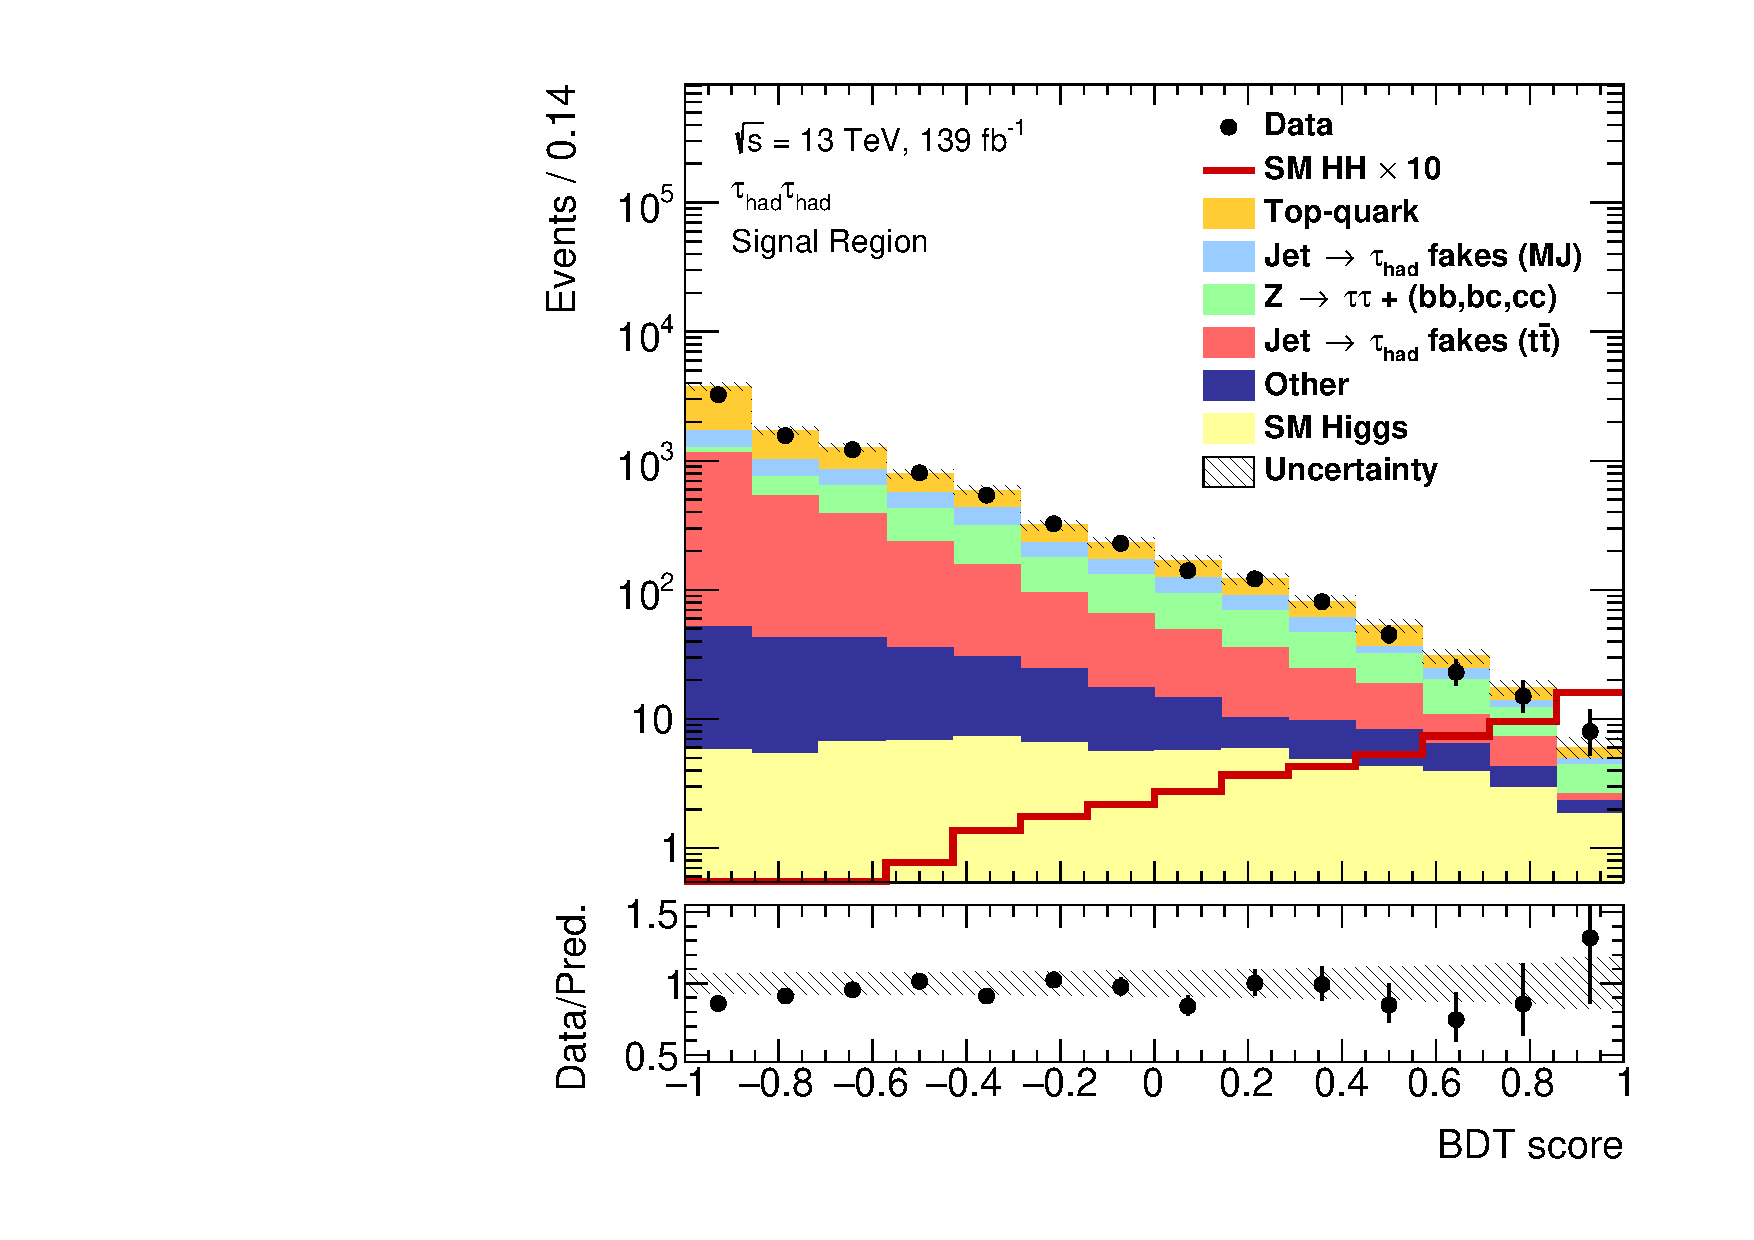
\includegraphics[width=0.6\textwidth]{mva/prefit/Region_BMin0_incJet1_distSMBDT_J2_Y2015_DLLOS_T2_SpcTauHH_L0_Prefitlog}

  \caption{Distribution of the BDT score used to select the SM \HH
    signal in the signal region of the \hadhad channel prior to the
    maximum likelihood fit. The uncertainty bands include all
    statistical and systematic uncertainties of the background
    model. The normalisation of the SM \HH signal is scaled by a
    factor of 10 for illustration purposes. The choice of binning for
    the histograms will be discussed in~\Cref{sec:binning_alg}.}
  \label{fig:mva_smbdt_prefit}
\end{figure}

The sensitivity to the SM \HH signal is driven by the last bins of the
BDT score histogram.  The expected number of signal (background)
events in the two most signal-like bins is 2.6 (24) out of 5.6 (9200)
events entering the signal region. The selection of the two most
signal-like bins provides a background rejection of
$1 / \varepsilon_{\text{b}} \approx 380$ while selecting almost half
of the signal events.

The single largest background in the last two BDT score bins, with an
expectation of 6.9 events, is associated production of
$\PZ \rightarrow \tautau$ with jets originating from heavy-flavour
quarks. The production of single Higgs bosons represents the second
most abundant background in the signal-like bins of the final
discriminant. The primary source being~$\PHiggs \rightarrow \tautau$
with approximately equal contribution from the \ggF, $\PZ\PHiggs$, and
$\ttbar\PHiggs$ production modes. A small fraction of
\SI{15}{\percent} is originating from $\PHiggs \rightarrow \bbbar$ in
associated production with a \PZ boson. The kinematic properties of
single Higgs boson production, particularly in the $Z\PHiggs$ mode, is
similar to the non-resonant \HH signal and largely limited by the
\PHiggs-system mass reconstruction performance such that about 1 in 15
single Higgs boson events in the signal region are selected into one
of the two most signal-like bins, yielding an expectation of 4.8
events. Other backgrounds populating the two most signal-like bins in
BDT score are originating from \ttbar (with \truetauhadvis in the
decay) with an expectation of 4.6 events and \jettotauhadvis from
multi-jet and \ttbar production with 2.2 and 3.4 expected events,
respectively. The signal and background yields including all
experimental and theoretical uncertainties will be summarised
in~\Cref{sec:statistical_analysis}.

The importance of input variables in the BDT can be estimated using
the \emph{permutation importance} technique. It is a method to inspect
the importance of input variables for predictions of a black box
estimator, derived from an importance measure introduced in
Ref.~\cite{breiman01} for random forests. To inspect the importance of
a feature in a given model, the feature's values are permuted over all
events and classes, breaking the relationship between the feature,
class labels, and other correlated input variables. The importance of
a given feature is estimated by measuring the degradation in the
quality of the model's predictions after permuting a given feature.

This technique measures the importance of a variable in a given model
which does not necessarily correspond to the importance of the
variable in solving the underlying predictive problem. In the presence
of highly collinear features this means that some importance can be
assigned to multiple related variables even if a strict subset of
variables contains the information relevant to the problem. This
effect needs to be considered when interpreting rankings based on the
permutation importance.

In~\Cref{tab:variable_importance_bdt} a ranking of the input variables
to the BDT for the SM \HH signal is shown based on the change in
ROC-AUC according to the permutation importance approach. The
\PHiggs-system masses are the most important inputs to the BDT,
contributing with approximately equal importance due to similar mass
reconstruction performance of \mMMC and \mBB. For the non-resonant SM
\HH search, the \HH-system mass is of lesser importance due to the
similarities of the \mHH spectra between signal and background
(cf.~\Cref{fig:mva_inputs}).

\begin{table}[htbp]
  \centering

  \caption{Importance of the input variables in the BDT measured as
    the change in ROC-AUC when permuting the values of a single
    variable over all events. The mean $\Delta\text{ROC-AUC}$ over 10
    permutations is displayed. The statistical uncertainty is below
    0.001 and therefore omitted. Variables are ordered from most to
    least important.}%
  \label{tab:variable_importance_bdt}

  % ["mBB", "mMMC", "mHH", "dRBB", "dRTauTau"]
% array([-0.08482375, -0.08992436, -0.03412635, -0.01212749, -0.03253109])
% (Pdb) p deltaROCAUC.mean(axis=1)
% array([-0.08560703, -0.09098586, -0.03392883, -0.01171693, -0.03247466])
% (Pdb) p deltaROCAUC.std(axis=1, ddof=1)
% array([0.00083227, 0.00054534, 0.00032627, 0.00020416, 0.00068158])

\begin{tabular}{lS}
  \toprule
  Variable & $\Delta\text{ROC-AUC}$ \\
  \midrule
  \mMMC & -0.090 \\
  \mBB & -0.085 \\
  \mHH & -0.034 \\
  \dRtautau & -0.033 \\
  \dRbb & -0.012 \\
  \bottomrule
\end{tabular}

%%% Local Variables:
%%% mode: latex
%%% TeX-master: "../../phd_thesis"
%%% End:

\end{table}


\subsection{Extraction of Signals from Resonant \HH Production with
  PNNs in the \hadhad Channel}%
\label{sec:mva_pnn}

The search for resonant \HH production considers scalar resonances
with masses ranging from \SIrange{251}{1600}{\GeV}, probing a wide
range of kinematic configurations of final state
particles. Consequently, the joint probability density of the
discriminating variables for signal processes varies with the assumed
mass of the resonance. This is particularly visible in the marginal
distributions of \mHH, \dRtautau, and \dRbb, previously shown
in~\Cref{fig:mva_inputs} for three \mX hypotheses, where the overlap
between the signal and background spectra changes as \mX is
varied. For optimal signal sensitivity for all assumed \mX, this
dependency should be exploited.

Using multivariate classifiers for signal extraction, one possible
method of incorporating the \mX dependency of the classification
problem is to train a classifier for every signal hypothesis. In this
approach multiple classification tasks are solved in isolation,
ignoring the more general classification problem. This was previously
explored in Ref.~\cite{HIGG-2016-16-witherratum} using BDTs.

An alternative approach is provided by parameterised classifiers where
the dependency of the prediction problem is incorporated during
training, thus solving it in a broader context. In particular,
Parameterised Neural Networks are used due to the ability of neural
networks to smoothly approximate large classes of continuous
functions~\cite{Baldi:2016fzo}. As a result of these properties, it is
shown in Ref.~\cite{Baldi:2016fzo} that PNNs are able to interpolate
the classification task to parameter values not seen in training. It
is also suggested that parameterised classifiers may outperform
approaches using one classifier per parameter value due to their
ability to solve the more general, parameter-dependent classification
problem.

In this search PNNs are implemented as feedforward neural networks
where, in addition to the five discriminating variables, the parameter
value specifying the classification task is provided as an input to
the network. During training, the value of the parameter is assigned
to be the generator-level \mX for signal events and random,
uninformative values for background events. Otherwise, PNNs are
amenable to the methods commonly employed to train non-parameterised
feedforward neural networks. At evaluation time the parameter value is
held fixed according to the classification problem to be solved.


\subsubsection{Implementation and Hyperparameter Optimisation}

The PNNs are trained using simulated signal events of 19 different
mass hypotheses of the scalar resonance. An additional point at
$\mX = \SI{375}{\GeV}$ was included at a later stage of the analysis
and was not part of the training and optimisation process. The
background processes considered in the training are the same as the
ones used for the non-resonant SM \HH search. Non-resonant SM \HH
production is not included as a background.
% Because it has not yet been observed
The signal event samples are combined, ensuring that every \mX
hypothesis contributes with the same total event weight to the
combined sample, subsequently normalising the combined signal and
background sample to have equal weight. The 5-fold CV approach is used
for model selection.

The training proceeds by minimising the binary cross-entropy loss
using stochastic gradient descent with momentum and exponential
learning rate decay. As part of the training process, the
discriminating variables are centred and scaled by subtracting the
median and dividing by the interquartile range of the variable for
better conditioning of the loss minimisation. Similarly, the values of
the mass parameter are (linearly) transformed into $[0, 1]$. The
values of the mass parameter for background events is sampled from the
\mX distribution in the combined signal sample and is re-sampled after
every training epoch. The neural networks consist of multiple
fully-connected layers with ReLU activation~\cite{nair:relu}, except
for the final layer which uses sigmoid activation. The training is
implemented in \textsc{Keras}~\cite{keras} using the
\textsc{TensorFlow}~\cite{tensorflow2015-whitepaper} backend. Trained
PNN are evaluated using \textsc{lwtnn}~\cite{lwtnn}.

The PNN hyperparameters are optimised, following the approach
previously employed for the BDT, using a random grid search with
nested cross-validation. The parameter grid is defined
in~\Cref{tab:hyperparameter_grid_pnn}. To reduce the dimensionality of
the hyperparameter space, the number of nodes in the hidden layers
except for the first and last hidden layers are required to be the
same.

\begin{table}[htbp]
  \centering

  \caption{Parameter values used to define the grid of hyperparameters
    considered for the optimisation of the PNN
    configuration. Parameters marked with $*$ and $\dagger$ are only
    applicable when the number of hidden layers is larger than 1 and
    2, respectively. The underlined values show the final PNN
    configuration after hyperparameter optimisation.}%
  \label{tab:hyperparameter_grid_pnn}

  \begin{tabular}{ll}
  \toprule
  Hyperparameter & Values considered \\
  \midrule
  Epochs & 50, 100, \underline{200}, 400 \\[0.1em]
  Batch size & 64, \underline{128}, 256 \\[0.1em]
  Learning rate & 0.01, 0.02, 0.05, 0.1, \underline{0.2} \\[0.1em]
  Learning rate decay & $10^{-6}$, \underline{$10^{-5}$}, $10^{-4}$, $10^{-3}$ \\[0.1em]
  Number of hidden layers & 1, 2, 3, \underline{4}, 5 \\[0.1em]
  Layer size (first hidden layer) & 16, 32, 64, \underline{128} \\[0.1em]
  Layer size (last hidden layer$^*$) & \underline{16}, 32, 64, 128 \\
  Layer size (other hidden layers$^\dagger$) & 16, 32, 64, \underline{128} \\[0.1em]
  \bottomrule
\end{tabular}

%%% Local Variables:
%%% mode: latex
%%% TeX-master: "../phd_thesis"
%%% End:

\end{table}

No clear choice of optimisation metric exists to evaluate a continuum
of related classification task. For simplicity, the ROC-AUC of the PNN
when performing binary classification of a resonant signal with
$\mX = \SI{325}{\GeV}$ against the background is chosen. This choice
is motivated by the strength of the $\PX \to \HH \to \bbtautau$ search
channel in an intermediate mass range of the scalar resonance from
approximately \SI{300}{\GeV} to \SI{600}{\GeV} compared to the \bbyy
and \bbbb channels which are expected dominate the low and high \mX
signal sensitivity, respectively. In the \hadhad channel, background
events with \mHH around \SI{325}{\GeV} are most abundant
(cf.~\Cref{fig:mva_inputs}) and therefore a value of \mX at the lower
end of the range is selected for optimisation.

About 1600 unique configurations of the PNN are tested, the 400
highest ranking ones in ROC-AUC showing compatible performance in
terms of the performance estimate obtained from CV. A single
configuration is obtained by choosing the best performing parameter
set in CV on even-numbered events and using the same configuration for
odd-numbered events. The chosen configuration, underlined
in~\Cref{tab:hyperparameter_grid_pnn}, has a ROC-AUC in 5-fold CV of
\num{0.9764 +- 0.0009} on even- and \num{0.9754 +- 0.0009} on
odd-numbered events.\footnote{On the dataset with odd-numbered events
  the chosen configuration is the 54\textsuperscript{th} highest
  ranking one in terms of the ROC-AUC. For comparison, the highest
  ranking model on odd-numbered event has a ROC-AUC of \num{0.9761 +-
    0.0020}, showing compatible performance with the chosen
  configuration.} The PNN are then re-fit on all five folds of the
inner CV separately for even- and odd-numbered events.

\subsubsection{Evaluation and Variable Importance}

\Cref{fig:pnn_score_prefit} shows the PNN score after evaluation on
withheld data in the signal region of the \hadhad channel for three
different values of the mass parameter. In each case the signal of
interest, resonant \HH production with \mX equal to the PNN mass
parameter, is populating the high PNN score bins. The background
processes contributing to the most signal-like bins depend on the
classification task that is solved by the PNN. At low mass
($\mX \approx {300}{\GeV}$) the dominant background is \ttbar with
both true- and \faketauhadvis constituting about \SI{80}{\percent} of
the total background with a small contribution from multi-jet.  The
background composition in the intermediate mass range
($\mX \approx \SI{500}{\GeV}$) is similar to the case of non-resonant
\HH production in the SM which has a mean reconstructed \mHH of about
\SI{500}{\GeV} after the signal region selection. For high mass
resonances, the most relevant backgrounds are the production of
$\PZ \to \tautau$ in association with jets from $b$- or $c$-quarks.

\begin{figure}[htbp]
  \centering

  \begin{subfigure}[t]{.49\textwidth}
    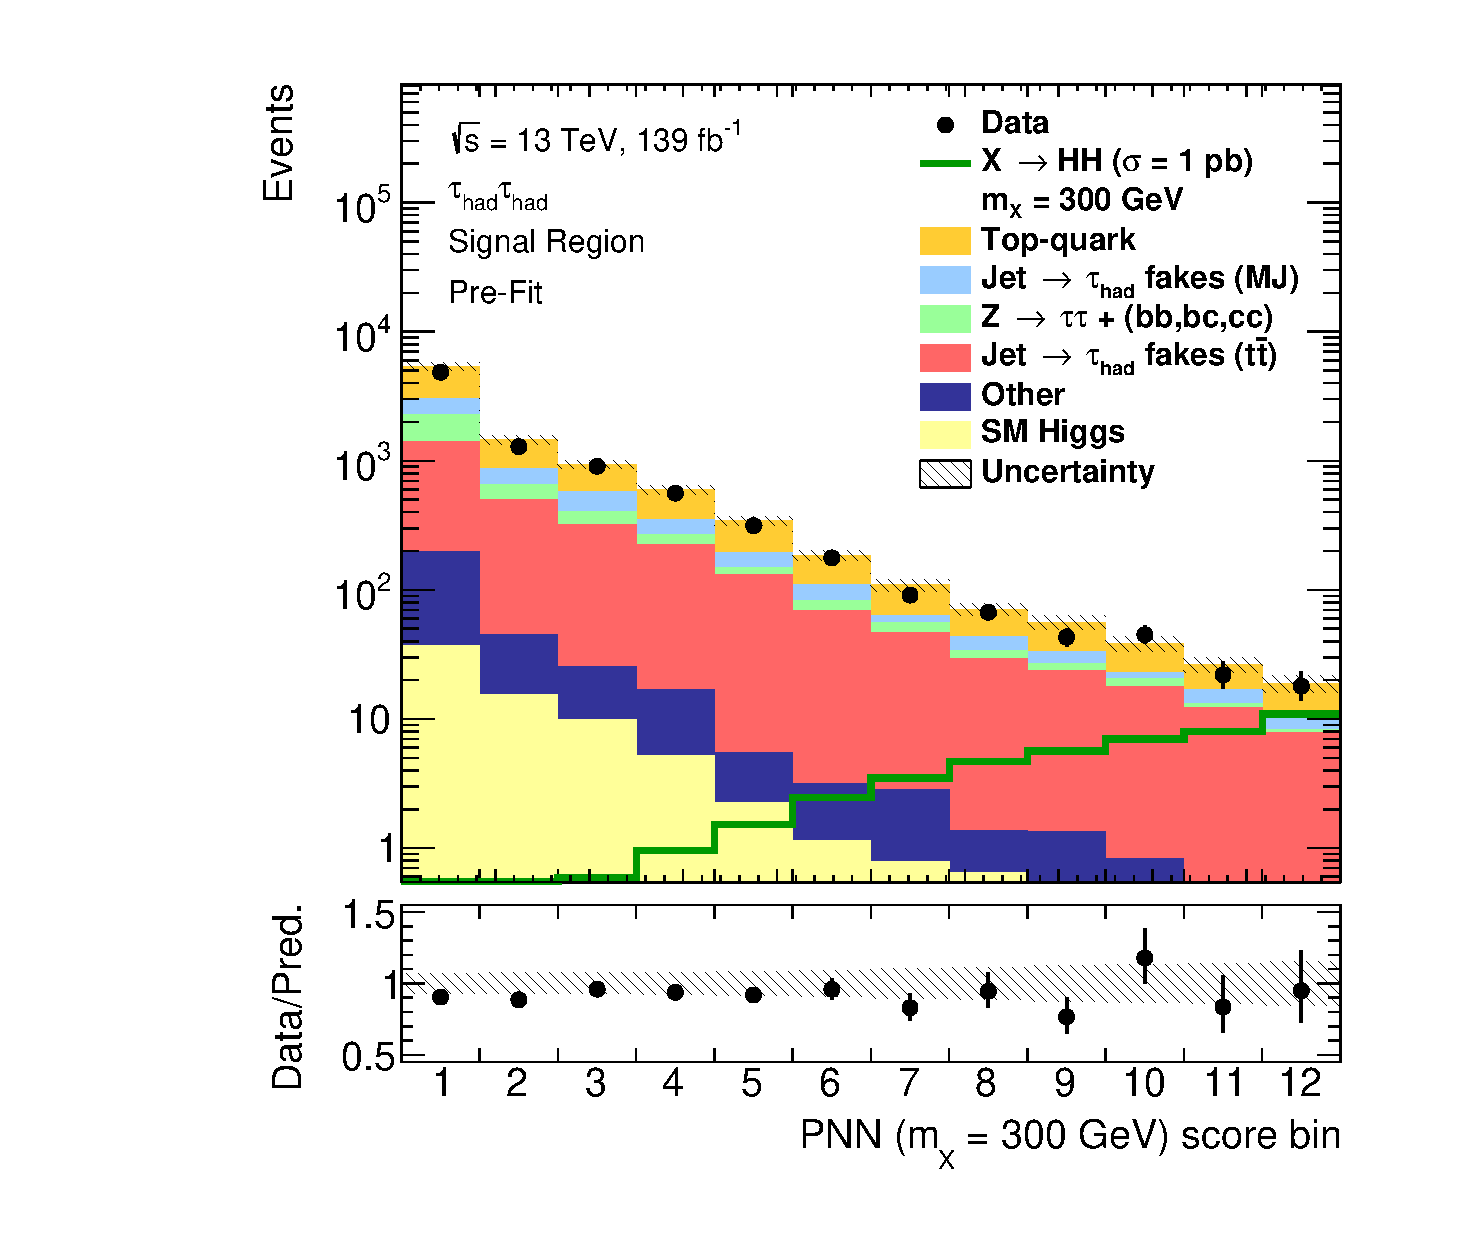
\includegraphics[width=\textwidth]{mva/prefit/Region_BMin0_incJet1_distPNN300_J2_Y2015_DLLOS_T2_SpcTauHH_L0_Prefit_logy}
    \caption{}
    \label{fig:pnn_score_prefit_300}
  \end{subfigure}\hfill%
  \begin{subfigure}[t]{.49\textwidth}
    \centering
    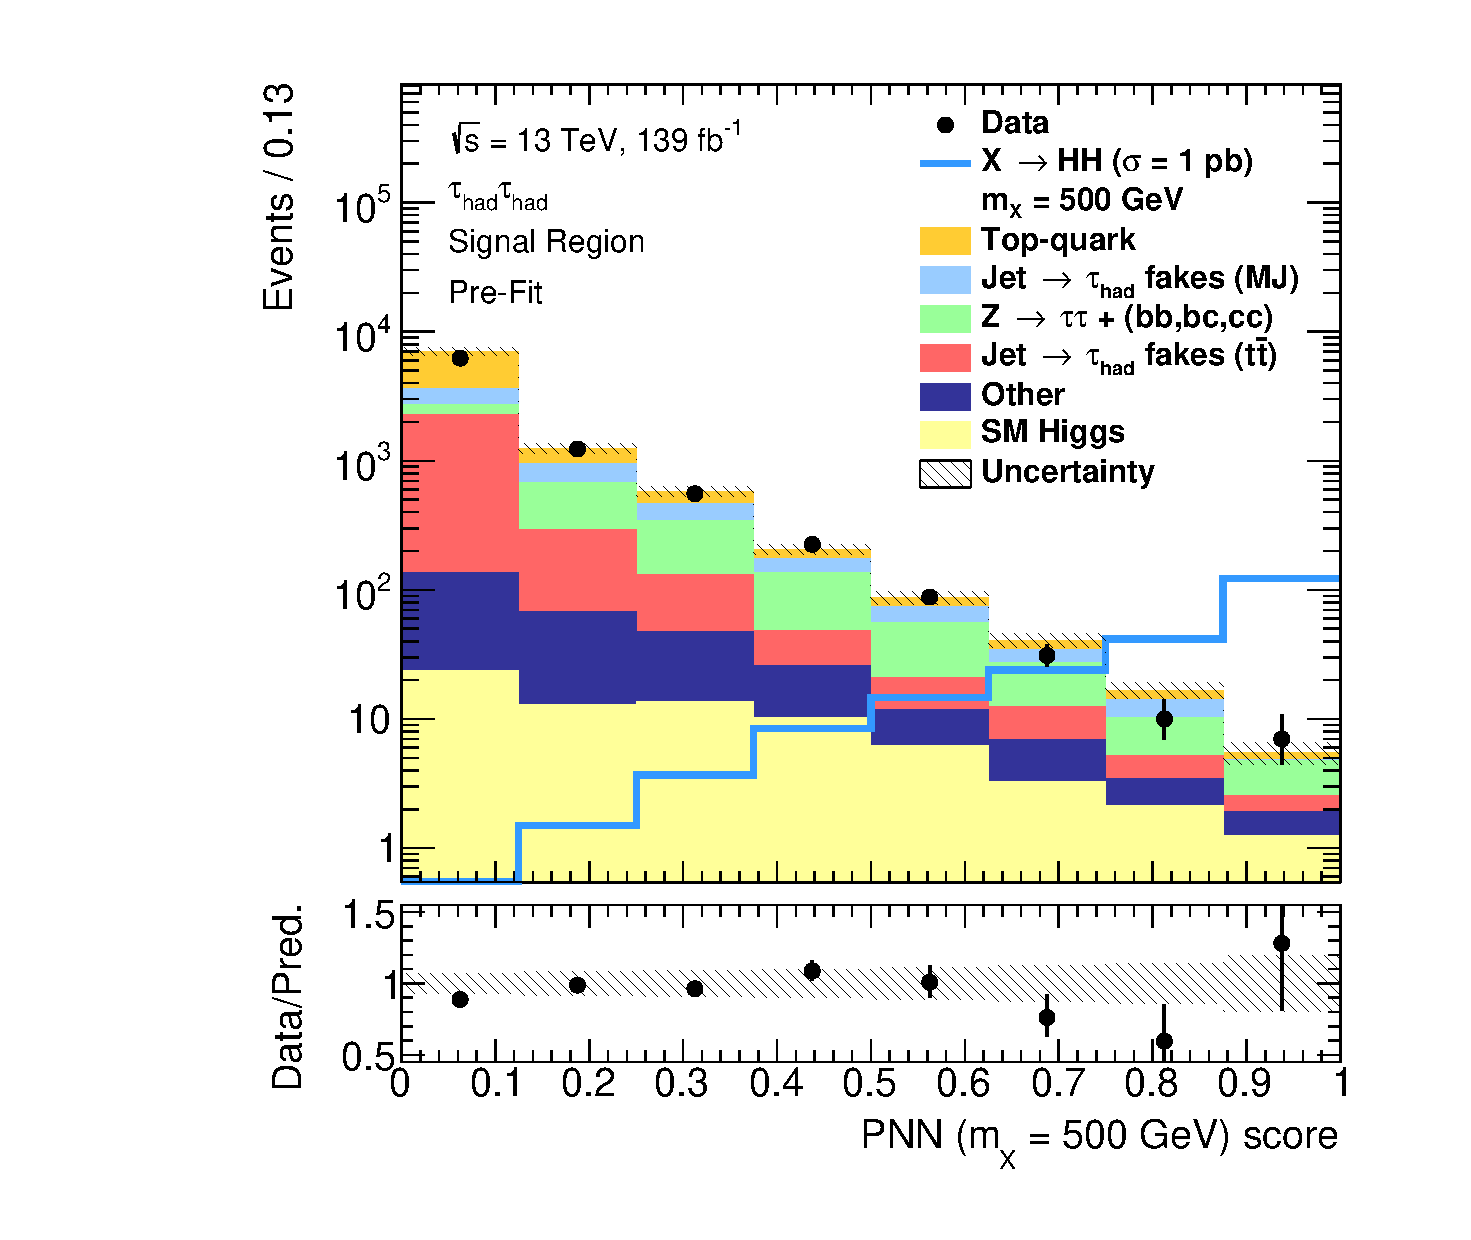
\includegraphics[width=\textwidth]{mva/prefit/Region_BMin0_incJet1_distPNN500_J2_Y2015_DLLOS_T2_SpcTauHH_L0_Prefit_logy}
    \caption{}
    \label{fig:pnn_score_prefit_500}
  \end{subfigure}

  \begin{subfigure}[t]{.49\textwidth}
    \centering
    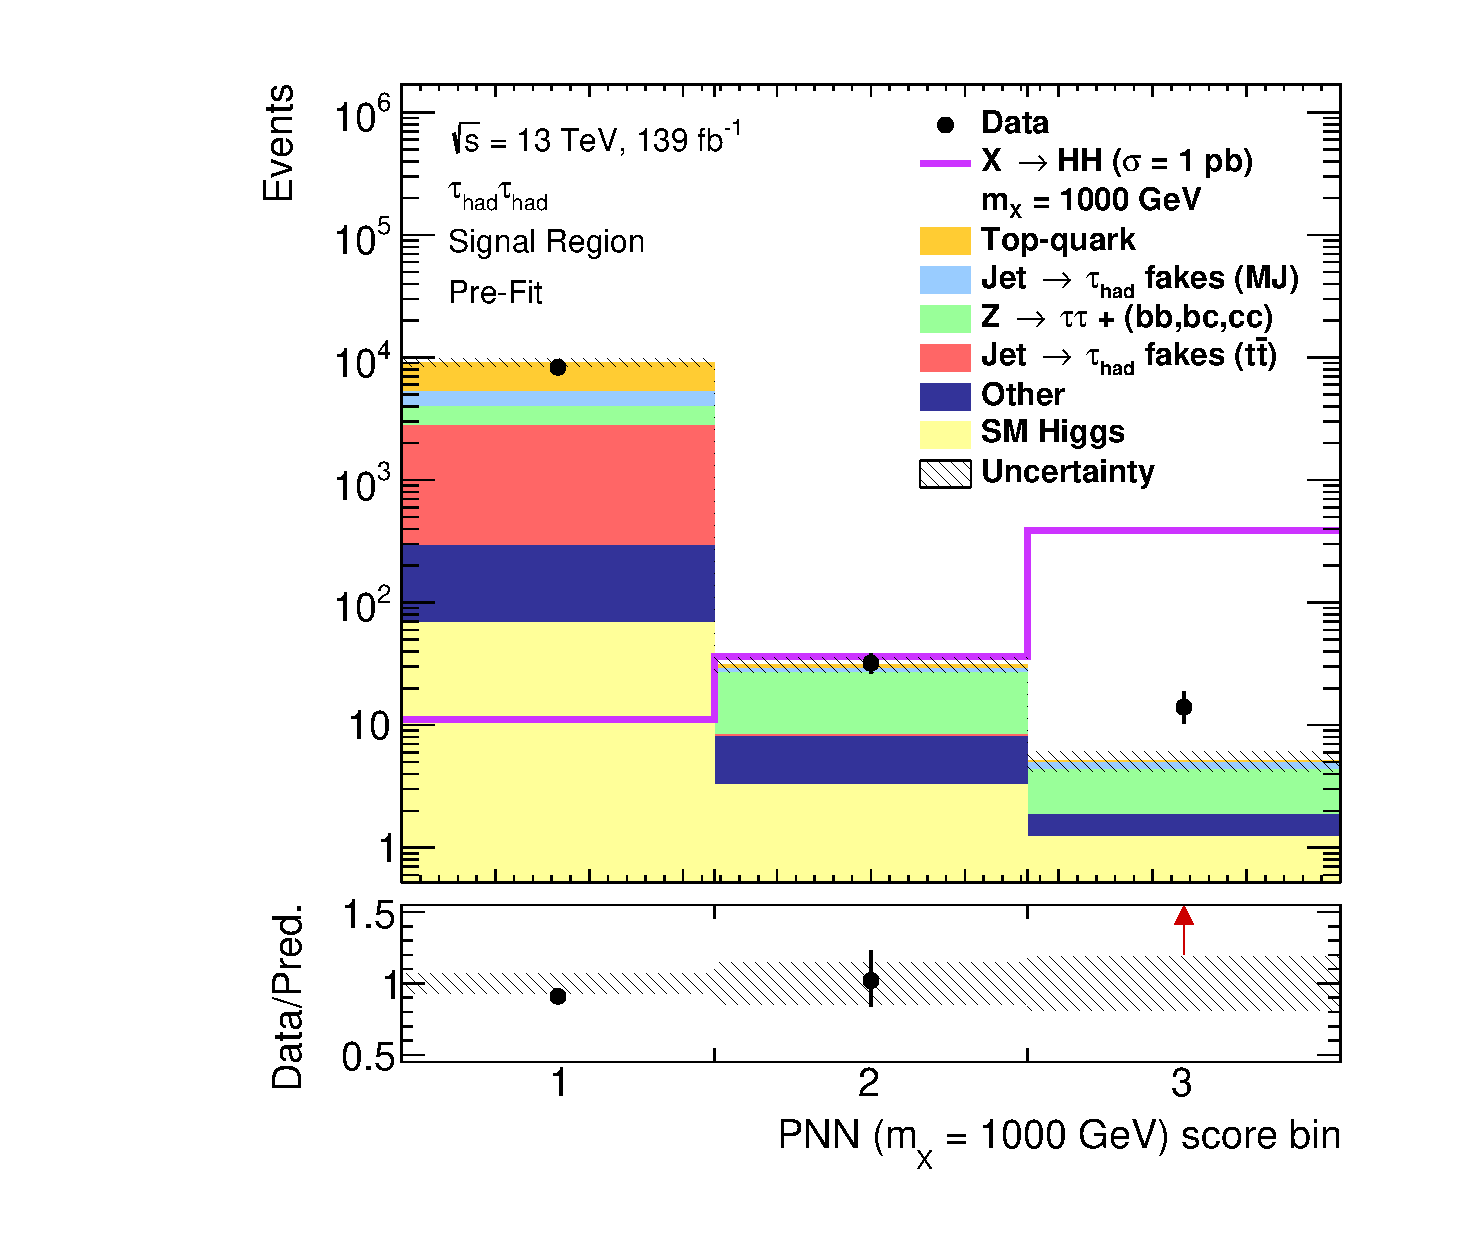
\includegraphics[width=\textwidth]{mva/prefit/Region_BMin0_incJet1_distPNN1000_J2_Y2015_DLLOS_T2_SpcTauHH_L0_Prefit_logy}
    \caption{}
    \label{fig:pnn_score_prefit_1000}
  \end{subfigure}

  \caption{Distribution of the PNN score evaluated with PNN mass
    parameters set to \SI{300}{\GeV} (a), \SI{500}{\GeV} (b), and
    \SI{1000}{\GeV} (c) prior to the fit.  The signal overlay is
    normalised to
    $\sigma(\Pproton\Pproton \to \PX \to \HH) =
    \SI{1}{\pico\barn}$. The choice of binning and excess of data in
    the most signal-like bin of the PNN ($\mX = \SI{1000}{\GeV}$)
    score will be discussed in \Cref{sec:statistical_analysis}.}%
  \label{fig:pnn_score_prefit}
\end{figure}

The previously discussed properties of PNN, the ability to solve a
continuously varying classification task parameterised by \mX and the
ability to interpolate to values of \mX not seen during training, are
investigated. For this, a performance metric is defined by binning the
PNN score for a given value of the mass parameter using an algorithm
that optimises the signal sensitivity while obeying certain
constraints. The binning algorithm will be formally introduced
in~\Cref{sec:binning_alg} for the statistical analysis of the results
of this search.
% The performance of the PNN is evaluated by binning its
% output score for a given value of the parameter using the algorithm
% also used for the statistical interpretation of the final results. The
% binning algorithm, which will be formally introduced
% in~\Cref{sec:binning_alg}, aims optimise the signal sensitivity while
% obeying constraints on the statistical uncertainty of the background
% estimate and the expected number of events in each bin.
The expected signal significance is approximated, assuming independent
Poisson counting experiments without uncertainties on the background
predictions, as~$\nu_\text{s} / \sqrt{\nu_\text{b}}$ for every bin,
where $\nu_\text{s}$ and $\nu_\text{b}$ is the expected number of
signal and background events, respectively. A combined significance is
obtained by adding the bin-wise significances in quadrature.

% Ability to handle multiple classification tasks
The combined significance is used in~\Cref{fig:pnn_detuning} to
inspect the change in signal sensitivity for a given benchmark signal
as the PNN mass parameter is varied. The largest expected significance
is obtained when the mass parameter is set close to the resonance mass
of the signal hypothesis.
% Ability to interpolate
In~\Cref{fig:pnn_interpolation} the ability of PNNs to interpolate to
classification tasks that were not part of the training is shown. The
signal significance is compared between a PNN excluding and including
a given signal hypothesis in training. The comparison shows similar
performance in both cases. This property motivates the use of PNNs
also for resonance masses that were not part of the training, and was
exploited to include an additional signal with $\mX = \SI{375}{\GeV}$
without retraining of the PNNs. % Why was it added? -> potential gap
% in sensitivity
Finally, the performance of the PNNs is compared to a strategy of
using dedicated BDTs for every signal mass hypothesis. The comparison
is performed for resonance masses of \num{300}, \num{500}, and
\SI{1000}{\GeV} using BDTs that are optimised following the approach
used for the BDTs in the SM \HH search. For these three values of \mX,
the use of PNNs improves the expected signal significance by
\SI{22}{\percent}, \SI{9}{\percent}, \SI{4}{\percent}, respectively,
over an approach of using dedicated classifiers.

\begin{figure}[htbp]
  \centering

  \begin{subfigure}[t]{.49\textwidth}
    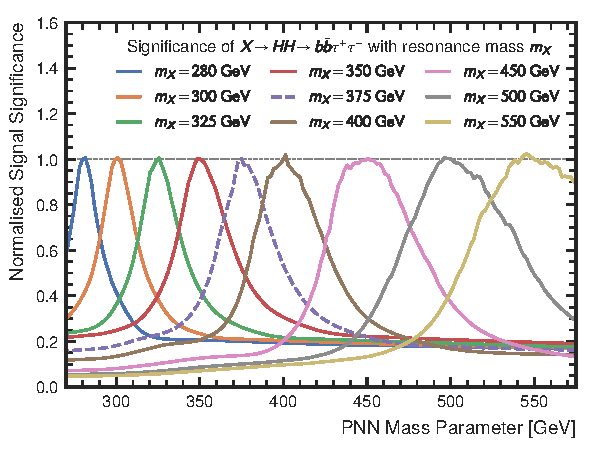
\includegraphics[width=\textwidth]{mva/detuning}
    \caption{Response of final PNN configuration used in the search
      for resonant production of \HH.}
    \label{fig:pnn_detuning}
  \end{subfigure}\hfill%
  \begin{subfigure}[t]{.49\textwidth}
    \centering
    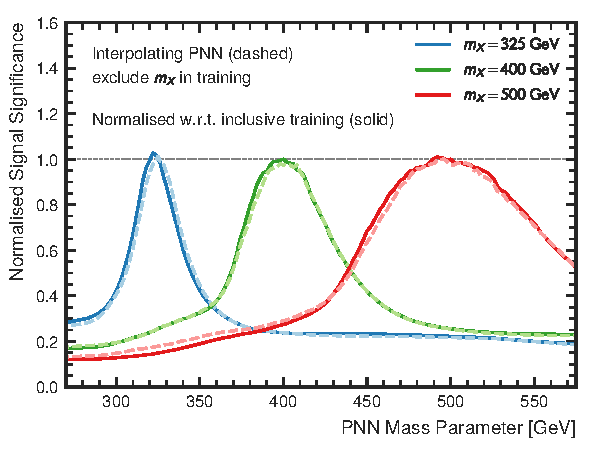
\includegraphics[width=\textwidth]{mva/interpolation}
    \caption{Comparison of PNN before hyperparameter optimisation when
      including (solid) and excluding (dashed) certain resonance
      masses in training.}
    \label{fig:pnn_interpolation}
  \end{subfigure}

  \caption{Expected signal significance of a scalar resonance with
    mass \mX as a function of the PNN mass parameter. The significance
    is estimated by binning the PNN score for a given value of the
    parameter and adding the Asimov significance of all bins in
    quadrature. Only statistical uncertainties are considered. The
    curves are normalised such that the significance is 1 when the PNN
    mass parameter is equal to \mX of the hypothesis under
    test. Dashed lines correspond to signal mass hypotheses not
    included in the PNN training.}
  \label{fig:pnn_properties}
\end{figure}

A ranking of the variable importance is provided
in~\Cref{tab:pnn_ranking} following the permutation importance
approach introduced previously. The \PHiggs-system masses continue
being important discriminants to reject backgrounds relevant for
searches of resonances in the low to intermediate mass range. The
reconstructed mass of the \HH-system provides an important
discriminant over the entire range of considered resonance masses,
becoming the highest ranked PNN input for~$\mX > \SI{500}{\GeV}$.

\begin{table}[htbp]
  \centering

  \caption{Permutation importance of the input variables to the PNN
    measured as the change in ROC-AUC (for the binary classification
    task between a signal with mass \mX and total background) when
    permuting the values of a single variable over all events. The
    mean $\Delta\text{ROC-AUC}$ over 10 permutations is displayed. The
    statistical uncertainty is below 0.002 for (a) and 0.001 for (b)
    and (c) and thus omitted.  Variables are ordered in in descending
    importance.}%
  \label{tab:pnn_ranking}

  \begin{subtable}[t]{.33\textwidth}
    \centering
    \subcaption{$\mX = \SI{300}{\GeV}$}
    \renewcommand{\arraystretch}{1.12}
    % # PNN300
% Bootstrap original: 0.97844 +- 0.00052
% # ['dRTauTau', 'dRBB', 'mMMC', 'mBB', 'mHH']
% 0,-0.12258,0.00097
% 1,-0.02916,0.00061
% 2,-0.33487,0.00105
% 3,-0.31694,0.00116
% 4,-0.16744,0.00138

\begin{tabular}{lS}
  \toprule
  Variable & {$\Delta\text{ROC-AUC}$} \\
  \midrule
  \mMMC & -0.335 \\
  \mBB & -0.317 \\
  \mHH & -0.167 \\
  \dRtautau & -0.123 \\
  \dRbb & -0.029 \\
  \bottomrule
\end{tabular}

%%% Local Variables:
%%% mode: latex
%%% TeX-master: "../../phd_thesis"
%%% End:

  \end{subtable}%
  \begin{subtable}[t]{.33\textwidth}
    \centering
    \subcaption{$\mX = \SI{500}{\GeV}$}
    \renewcommand{\arraystretch}{1.12}
    % # PNN500
% Bootstrap original: 0.99498 +- 0.00019
% # ['dRTauTau', 'dRBB', 'mMMC', 'mBB', 'mHH']
% 0,-0.01054,0.00031
% 1,-0.00506,0.00016
% 2,-0.17587,0.00073
% 3,-0.18303,0.00108
% 4,-0.17058,0.00087

\begin{tabular}{lS}
  \toprule
  Variable & {$\Delta\text{ROC-AUC}$} \\
  \midrule
  \mBB & -0.183 \\
  \mMMC & -0.176 \\
  \mHH & -0.171 \\
  \dRtautau & -0.011 \\
  \dRbb & -0.005 \\
  \bottomrule
\end{tabular}


%%% Local Variables:
%%% mode: latex
%%% TeX-master: "../../phd_thesis"
%%% End:

  \end{subtable}%
  \begin{subtable}[t]{.33\textwidth}
    \centering
    \subcaption{$\mX = \SI{1000}{\GeV}$}
    \renewcommand{\arraystretch}{1.12}
    % # PNN1000
% Bootstrap original: 0.99944 +- 0.00004
% # ['dRTauTau', 'dRBB', 'mMMC', 'mBB', 'mHH']
% 0,-0.00734,0.00013
% 1,-0.00180,0.00005
% 2,-0.00622,0.00010
% 3,-0.00834,0.00014
% 4,-0.18749,0.00086

\begin{tabular}{lS}
  \toprule
  Variable & {$\Delta\text{ROC-AUC}$} \\
  \midrule
  \mHH & -0.187 \\
  \mBB & -0.008 \\
  \dRtautau & -0.007 \\
  \mMMC & -0.006 \\
  \dRbb & -0.002 \\
  \bottomrule
\end{tabular}


%%% Local Variables:
%%% mode: latex
%%% TeX-master: "../../phd_thesis"
%%% End:

  \end{subtable}

  % \begin{subtable}[t]{.33\textwidth}
  %   \centering
  %   %% # PNN700
% Bootstrap original: 0.99831 +- 0.00006
% # ['dRTauTau', 'dRBB', 'mMMC', 'mBB', 'mHH']
% 0,-0.00992,0.00021
% 1,-0.00353,0.00009
% 2,-0.04351,0.00042
% 3,-0.04608,0.00039
% 4,-0.19180,0.00080

\begin{tabular}{lS}
  \toprule
  Variable & {$\Delta\text{ROC-AUC}$} \\
  \midrule
  \mHH & -0.192 \\
  \mBB & -0.046 \\
  \mMMC & -0.044 \\
  \dRtautau & -0.010 \\
  \dRbb & -0.004 \\
  \bottomrule
\end{tabular}


%%% Local Variables:
%%% mode: latex
%%% TeX-master: "../../phd_thesis"
%%% End:

  %   \subcaption{$\mX = \SI{700}{\GeV}$}
  % \end{subtable}
\end{table}

The sensitivity of the signal extraction method to the mass of the
resonance decreases with increasing \mX, as is indicated by the width
of the curves in \Cref{fig:pnn_detuning}. This decrease in mass
sensitivity has two primary sources. First, the mass resolution of the
reconstructed \mHH increases approximately linearly with \mX. Second,
the PNN has high separation power between events from background
processes and resonant \HH production at high mass.\footnote{The
  discrimination power of the PNN as a function of the \mX of the
  signal hypothesis is shown in \Cref{fig:pnn_rocauc_vs_mx} in the
  appendix.}  Due to the large separation power, the mass sensitivity
in the high mass regime is limited by the width of bins in the high
PNN score region, the bin width being driven by constraints imposed on
the binning algorithm. In these cases, the signal extraction method
employed in this search shows worse mass sensitivity than suggested by
the resolution of the \mHH reconstruction itself. Consequently, the
approach of using the score of a multivariate classifier as a final
discriminant in this search is optimised for the discovery of a signal
as opposed to perform a measurement of the resonance mass.

% The width of the significance response of the PNN as the mass
% parameter is varied can serve to understand the sensitivity and
% specificity of the signal extraction method in distinguishing between
% different signal hypotheses. The response, previously shown
% in~\Cref{fig:pnn_detuning}, exhibits peaks of increasing width as the
% tested signal hypothesis increases in \mX. This is illustrated
% in~\Cref{tab:pnn_width} where intervals of the PNN parameter are given
% that yield signal significances exceeding \SI{75}{\percent} and
% \SI{50}{\percent} of the maximum for a given hypothesis. At very high
% masses of the resonance, the signal extraction method, while being
% highly sensitive, loses specificity to the signal hypothesis of
% interest.


% \begin{table}[htbp]
%   \centering

%   \caption{Intervals of the PNN mass parameter where a hypothesis test
%     of a signal with a given resonance mass in the PNN score
%     distribution would yield \SI{75}{\percent} (\SI{50}{\percent}) of
%     the expected significance at the maximum.}%
%   \label{tab:pnn_width}

%   % 50%
% [[ 285.67350152  317.7744856 ]
% [ 465.50033084  549.35961107]
% [ 631.87907996  826.11120662]
% [ 855.48442134 1301.9140074 ]]

% 75%
% [[ 292.59952886  309.62423479]
% [ 479.17777504  530.05496437]
% [ 653.27841442  786.72796647]
% [ 885.67288997 1201.38754502]]

{
  \newcolumntype{G}{>{\centering\arraybackslash}m{4.3cm}}
  \begin{tabular}{lGG}
    \toprule
    & \multicolumn{2}{c}{PNN parameter [\si{\GeV}] interval where significance exceeds} \\
    \cmidrule{2-3}
    {Resonance mass\hspace{1em}} & \SI{75}{\percent} of maximum & \SI{50}{\percent} of maximum \\
    \midrule
    \SI{300}{\GeV} & $[293, \phantom{1}310]$ & $[286, \phantom{1}318]$ \\
    \SI{500}{\GeV} & $[479, \phantom{1}530]$ & $[466, \phantom{1}549]$ \\
    \SI{700}{\GeV} & $[653, \phantom{1}787]$ & $[632, \phantom{1}826]$ \\
    \SI{1000}{\GeV} & $[886, 1200]$ & $[855, 1300]$ \\
    \bottomrule
  \end{tabular}
}

%%% Local Variables:
%%% mode: latex
%%% TeX-master: "../phd_thesis"
%%% End:

% \end{table}

% % Example
% This effect can be illustrated by considering the hypothesis of a
% signal with $\mX = \SI{1000}{\GeV}$. The score of the PNN evaluated
% with a mass parameter of \SI{1000}{\GeV} will yield a hypothesis test
% with an expected significance close to the maximum. However, tests
% performed using PNN mass parameter values of \num{900}, \num{1100},
% and \SI{1200}{\GeV}, are expected to be significant at a level of
% \SI{75}{\percent} of the maximum.

% Explanation
% The reason for the reduced specificity in selecting signals with high
% \mX primarily originates from two sources. Firstly, the experimental
% mass resolution presents a bound in distinguishing between competeting
% signal hypotheses. Secondly and more pertinent to the choice of
% analysis strategy, the approach of using binary classification, even
% when parametrised in \mX, does not guarantee optimal discrimination
% between signal hypotheses. A resulting side-effect is that the
% intervals presented~\Cref{tab:pnn_width} show an asymmetry towards
% larger values of the mass parameter, which originates from the
% exponentially falling background density\footnote{Neural networks
%   approximate probabilistic classification based on the ratio of
%   signal and background densities. An univariate example is the
%   presence of a symmetric signal peak on a falling background
%   spectrum. A classification rule based on the density ratio will be
%   asymmetric with respect to the centre of symmetry of the signal
%   density.} in \mHH\todo{Strong statement given this is MVA.}. The
% approach of using binary classification in this search is primiarily
% optimised for discovery as opposed to the measurement of the
% properties of the resonance.


%%% Local Variables:
%%% mode: latex
%%% TeX-master: "../../phd_thesis"
%%% End:
